\documentclass{article}
\usepackage{graphicx} % Required for inserting images
\usepackage{float}
\usepackage[table,xcdraw]{xcolor}
\usepackage{array}
\usepackage{spverbatim}

\begin{document}
\begin{figure}[t]
    
\includegraphics[scale=0.8]{logo_polimi.png}
    \centering
\end{figure}

\begin{titlepage}
    \newcommand{\HRule}{\rule{\linewidth}{0.5mm}}
    \center
	\textsc{\Large SOFTWARE ENGINEERING II}\\[0.5cm]
	
	\HRule\\[0.4cm]
	    {\huge \textsc{Students\&Companies - \\Requirements Analysis and Specification Document}}\\[0.4cm]
    \HRule\\[1.5cm]
	
	\begin{minipage}{1\textwidth}
		\begin{flushleft}
			\large
			\textit{Authors}\\
			Priuli \textsc{Elia}\\
			Viceconti \textsc{Veronica}\\
			Zuccoli \textsc{Marco}\\
		\end{flushleft} 
         \hspace*{\fill} 21 Dicember 2024 \newline
         \hspace*{\fill} Version 1
	\end{minipage}
\end{titlepage}

\newpage
\tableofcontents
\newpage
\section{Introduction}
\subsection{Purpose}
When students reach the point where they can pursue internships, it can be a critical time due to numerous challenges such as finding opportunities that also match their interests.
For example, a lot of time is wasted looking for these opportunities because there are no notifications or updates on available internships.
On the other hand, companies, very often, struggle to find (or don't have access to) the proper information about potential student/candidates they are looking for the position, which once again leads to wasted of time.
It's with these issues in mind that S\&C steps in, allowing students to search for internships they are interested in while helping companies to create internship opportunities, specifying their requirements and terms.

\subsubsection{Goals}
\begin{enumerate}
    \item Make it easier for students to find internships
    \item Make it easier for companies to find students
    \item Support interviews 
    \item Monitoring internships progress 
\end{enumerate}

\subsection{Scope}

\subsubsection{World Phenomena}
[WP1] Creation of projects for internships\newline
[WP2] Students undertake internships in companies\newline
[WP3] Companies supervise students during the internship\newline
[WP4] Students form opinions about the company where they intern\newline
[WP5] Companies form opinions about the students\newline
[WP6] Companies contact potential candidates\newline

\subsubsection{Shared Phenomena}

\textbf{World controlled} \newline
[SWC1] Internship publication by companies\newline
[SWC2] Student's application publication\newline
[SWC3] Students select the received match notifications\newline
[SWC4] Companies select the received match notifications\newline
[SWC6] Creation of interview forms by companies\newline
[SWC7] Universities review their students' feedback to manage complications\newline
[SWC8] Students update their CVs and/or preferences\newline
[SWC9] Companies update their projects and/or preferences\newline
[SWC10] Students independently search for internships\newline
[SWC11] Students submit internship complaints\newline
[SWC12] Companies submit internship complaints\newline

\textbf{Machine controlled}\newline
[SMC1] Request final internship feedback from students\newline
[SMC2] Request final internship feedback from companies\newline
[SMC3] Notify students when new compatible companies are available\newline
[SMC4] Notify universities upon the publication of a complaint\newline
[SMC5] Notify companies when new compatible students are available\newline
[SMC6] Provide suggestions to students on how to write their CV\newline
[SMC7] Provide suggestions to companies on how to publish their projects\newline

\subsubsection{Machine Phenomena}
[MP1] Mechanisms of various level of sophistication to match students with internships (from simple keyword searching, to statistical analyses based on final feedbacks made by students and companies)\newline
[MP2] Analysis of new student publications for companies\newline
[MP3] Analysis of new internship publications for students\newline
[MP4] Analysis of interviews to assist companies\newline

\subsection{Definitions, Acronyms, Abbreviations}
\subsubsection{Acronyms}
\begin{itemize}
    \item  S\&C:  Student\&Companies
    \item  CV: Curriculum Vitae
    \item HTTPS: HyperText Transfer Protocol over Secure Socket Layer
    \item CSRF: Cross-site Request Forgery 
    \item XSS: Cross-site scripting 
    \item MTFB: Mean Time Between Failures
    \item GDPR: General Data Protection Regulation
\end{itemize}
\subsection{Reference Documents}
RASD document A.Y. 2024/2025 given by the professor in the slides.

\subsection{Document Structure}
The document is divided into six sections, each with its unique focus, as outlined below.\newline \newline
\textbf{Introduction}: In the first section, we outline the project's goals, aims, and provide a succinct analysis of universal and shared phenomena. This section also incorporates a glossary of abbreviations and definitions necessary for understanding the issue.\newline \newline
\textbf{Overall Description}: The second section offers a detailed summary of the problem. It explores additional aspects of the domain and various scenarios involved, as well as addressing product and User attributes, assumptions, dependencies, and limitations.\newline \newline
\textbf{Specific Requirements}: The third section focuses on a thorough examination of the specific requirements. It provides comprehensive details about external interface requirements, functional specifications, and performance criteria.\newline \newline
\textbf{Formal Analysis Using Alloy}: The fourth section utilizes Alloy for conducting a formal analysis. The main aim of this chapter is to verify the correctness of the model described in the earlier sections. It emphasizes presenting the outcomes of the conducted verifications and key assertions.\newline \newline
\textbf{Effort Spent}: Section five details the individual contributions of each team member in creating this document.\newline \newline
\textbf{References}: The final section acts as a bibliography, listing the references and supplementary materials utilized in drafting this document.
\section{Overall Description}
\subsection{Product perspective}

\subsubsection{Scenarios} 

\newcounter{scenario}
\setcounter{scenario}{1}

\textbf{Scenario \thescenario: Account creation }  \newline
\textbf{Description}: A new user (student or company) that wants to find (or publish) an internship opportunity, access the platform on the specific page and inserts all the requested data. At this point the user account is created \newline
\newline
\stepcounter{scenario}
\textbf{Scenario \thescenario: Managing internships }  \newline
\textbf{Description}: A company accesses a section on the platform where it can: create/modify/remove an internship opportunity  (possibly facilitated by our application) and its students' preferences. When requested the company has to insert the requested data.
\newline
\newline
\stepcounter{scenario}
\textbf{Scenario \thescenario: Managing CV and internship preferences}  \newline
\textbf{Description}: The student access its personal page and insert/modify its CV (possibly facilitated by our application) and his Internships' preferences\newline
\newline
\stepcounter{scenario}
\textbf{Scenario \thescenario: Student search an Internship}  \newline
\textbf{Description}: The student accesses the platform, uses the search function to explore available internships based on their interests and skills, and submits an application for the internships they are interested in.
\newline
\newline
\stepcounter{scenario}
\textbf{Scenario \thescenario: Evaluation of Internship Opportunities for a Student}\newline
\textbf{Description}: The student receives a notification when a match is made or when the company they applied to responds to their application. If a match notification is received, the student has the option to accept or decline the internship.\newline
\newline
\stepcounter{scenario}
\textbf{Scenario \thescenario: Evaluation of a new student available for the internship}\newline
\textbf{Description}:  The company receives a notification when a student with a CV that matches the requirements is available, and can decide whether to accept or decline.
\newline
\newline
\stepcounter{scenario}
\textbf{Scenario \thescenario: Feedback during internship}\newline
\textbf{Description}:  The company and the student can provide feedback on the current progress of the internship in a dedicated section on the platform.\newline
\newline
\stepcounter{scenario}
\textbf{Scenario \thescenario: Manage selection process}\newline
\textbf{Description}: After receiving the applications, the company reviews the profiles of the interested students and selects some candidates for an interview. The company can use the platform to conduct the interviews.
\newline
\newline
\stepcounter{scenario}
\textbf{Scenario \thescenario: Feedback Post-Internship}\newline
\textbf{Description}: At the end of the internship, after receiving a feedback request from the platform, the student evaluates the training experience and the work environment, while the company assesses the student's performance.
\newline
\newline
\stepcounter{scenario}
\textbf{Scenario \thescenario: University monitor the student's internship}\newline
\textbf{Description}: Once the student starts the internship, the university must monitor the progress through the platform. If the student or the company reports any issues, the university receives a notification and can intervene to resolve the problem, managing communication between the student and the company or terminating the internship if necessary.\newline
\subsubsection{Domain class diagram}
\begin{figure}[H]
    \centering
    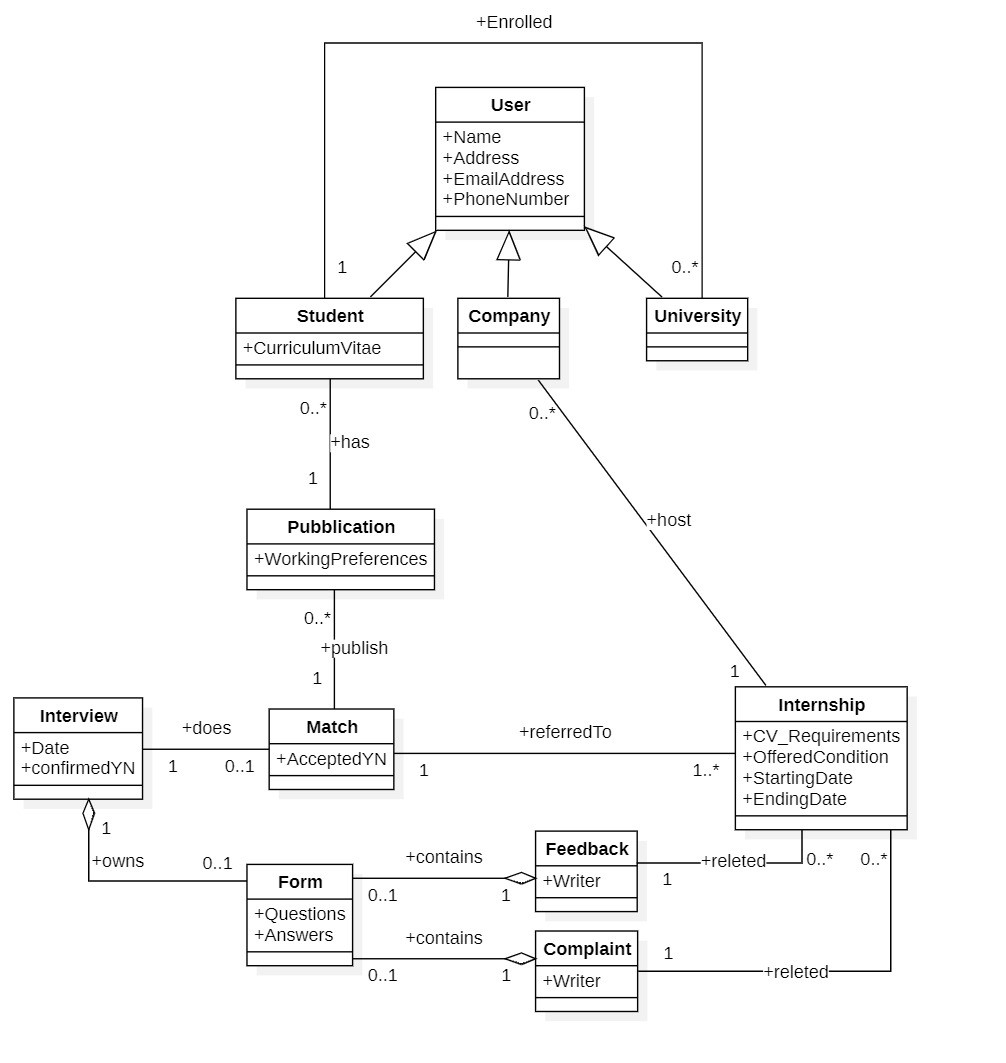
\includegraphics[width=1\linewidth]{ClassDiagram.jpg}
    \caption{Class Diagram}
    \label{fig:enter-label}
\end{figure}

\begin{enumerate}
    \item User: the class that represents the general entity that interact with the system. The sub-classes Student, Company and University better represent the different types of clients in the platform. Each of them is able to visualize different part of the system and carry out different operations on it. Students upload their CV, working preferences and browse the platform scanning for an internship. Companies publish internship opportunities. Both can write feedbacks, eventual complaints and accept or decline matches found by the platform. Finally, universities address the complaints related to internships involving their students.
    \item Publication: used to collect the student's information made available to compute eventual matches with internships. A student can have multiple publication because it will be possible to express different preferences. For example: Part time internship in software engineering and full time in computer security.
    \item Internship : Represents an internship available at a company
    \item Match: Class useful to connect the matches that the platform identifies between students and companies' internships. It contains the information about the acceptance. In particular its attribute "AcceptedYN" is "Yes" when both student and company accept the match.
    \item Interview: Represents the interaction between a company and a student during the interview process. It stores the questions asked during the interview and the corresponding answers provided by the student, which are manually entered into the system by the company representative. The system assists the company in designing and organizing the interview form, allowing all the necessary questions to be collected and structured efficiently. When the interview is done, the "ConfirmedYN" attribute is set and if it is set to "Yes", the Company has totally accepted the student and the internship can start. If it is set to "No", the Company doesn't accept the student and the Internship won't start.
    
    \item Form: A standard structure used to represent a set of questions and the corresponding answers. It's used both to structure an interview but also to collect feedbacks and complaints (in these case there's only one question)
    \item Complaint/Feedback : Used to collect feedbacks given both by companies and students about and ongoing internships. The first one is monitored by universities whereas the other ones are used to provide statistical data in order to improve the matching process 
    
    
\end{enumerate}
\subsubsection{State Diagram}
\begin{figure}[H]
    \centering
    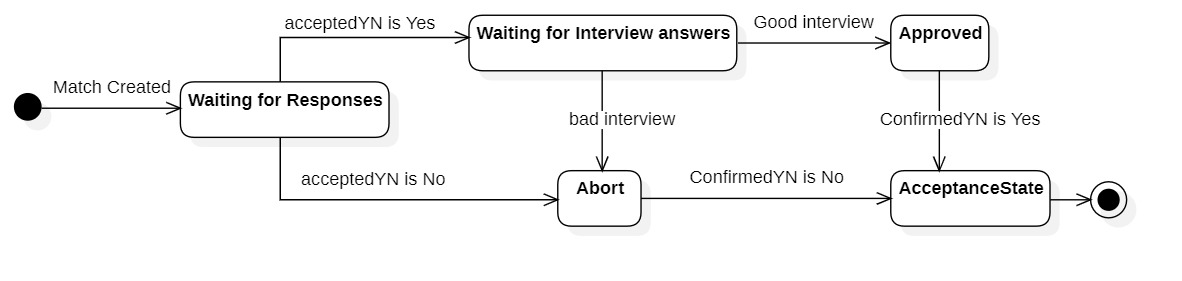
\includegraphics[width=1\linewidth]{StateDiagram.jpg}
    \caption{Match's state diagram}
    \label{fig:enter-label}
\end{figure}
Figure 2 illustrates the state flow of the match entities. When a new match is identified between a student and an internship, a Match entity is created. Initially, it remains in an Idle state, awaiting decisions from both parties (Company and Student).

If both the Company and Student accept the match—indicating mutual interest—it transitions to the Waiting for Interview Answers state. In this stage, the company conducts an interview with the student.

Upon completing the interview process, the company determines whether to proceed with the internship. If the company decides to move forward, the match transitions to the Approved state, signifying a successful pairing. In this context the AcceptYN in the match entity is set to YES and the internship starts.
Conversely, if the company decides not to proceed, or if either party initially declines the match, the process transitions to an Abort state, terminating the match.
\subsection{Product functions}
\textbf{Manage student information}\newline
It allows students, after creating their account, to create, update, and manage their profiles by entering details such as experiences, skills, abilities, and CV.\newline
\newline
\textbf{Manage company information}\newline
It allows companies, after creating their account, to create, update, and manage their profiles by entering details such as application domain, tasks to be performed, relevant adopted technologies and their terms, and the requirements they are looking for in students.\newline
\newline
\textbf{Analysis and matching generation}\newline
After the publication of profiles by students and companies, the system analyzes this data, enabling the creation of valid matches between the two.\newline
\newline
\textbf{Send notification to the users}\newline
After the creation of the profile, the system sends notifications to users to inform them about the following areas:
-New matches detected
-Acceptance/rejection of internship
-Student complaints to their university
\newline
\newline
\textbf{Support Interview and Selection Process}\newline
After the matching, the system assists companies in the interview and selection process. In particular, companies can prepare structured questionnaires to assess the students' qualifications and suitability for the position. The system allows the interviewer to fill in the questionnaire with the student's answers during the interview.\newline
\newline
\textbf{Feedback from users during the internship}\newline
After accepting the internship, users (students and companies) can use their profile during the experience to provide ongoing feedback regarding the progress of the internship. \newline
\newline
\textbf{Management and monitoring of the internship by universities}\newline
Universities have the ability to view their students' feedback from various companies and can terminate the internship if they find it necessary following particularly negative feedback.\newline
\newline
\textbf{Feedback and Improvement Recommendations from Users}\newline
At the end of an internship, users (students and companies) can leave feedback on the completed internship. The platform uses this data to provide improvement suggestions for the corresponding profiles (for example, making internship descriptions more attractive or offering tips to improve the CV).\newline
\newline

\subsection{User Characteristics}
There are mainly three types of user that interact with the platform: students, universities and companies.\newline

\subsubsection{Student}
The students in this system are primarily university students who are looking for internships to gain work experience. They can be graduates or undergraduates, with varying levels of knowledge, available for part-time or full-time positions, and seeking both paid and unpaid internships.

\subsubsection{Universities}
Universities are the institutions where students attend their faculties, and their role, through the system, is to monitor the development of internships and ensure that no issues arise between the two parties.

\subsubsection{Companies}
Companies are those looking for students to include in their workforce for internships. They can be small, medium, or large in size, with or without benefits, and may require specific skills from the students.

\subsection{Assumptions, dependencies and constraints}
\subsubsection{Domain Assumptions}
The following assumptions are made for the domain. They are properties or conditions that the system will take for granted.They must be checked to ensure a correct platform behaviour:\newline
[D1] The students have to be at the end of their career\newline
[D2] The CVs have to contain real data\newline
[D3] The companies have to public only available internship\newline
[D4] The student must have uploaded a CV in EU format to ensure the proper functioning of the application\newline
[D5] Students and companies must have an email for communication\newline
[D6] The student's email must be a university email\newline


\section{Specific Requirements}
\subsection{External Interface Requirements }
The application will be developed through a WebApp.
\subsubsection{User interfaces }
In order to use all the functionalities provided by the platform, it must have the following interfaces:
\begin{enumerate}
    \item Student : 
    \begin{enumerate}
        \item An interface that allows them to view their profile with all their information
        \item An interface that allows them to publish their preferences and CV
        \item An interface that allows them to view companies and their available internships  
        \item An interface to manage matches (accept, reject, or view their status)
        \item An interface to provide feedback and/or complaints
    \end{enumerate}
    \item Company  
    \begin{enumerate}
        \item An interface that allows them to view their profile with all their information
        \item An interface that allows them to publish their preferences and new internships
        \item An interface to manage matches (accept, reject, or view their status)
        \item An interface for managing interviews (creation, completion, acceptance, and rejection)
        \item An interface to provide feedback and/or complaints
    \end{enumerate}
    \item University
    \begin{enumerate}
        \item An interface to manage complaints and/or feedback from their students (including the option to prematurely terminate an internship)
    \end{enumerate}
Additionally, each user must have a login and sign-up page.
\end{enumerate}

\subsubsection{Hardware interface requirements}
As for hardware, a common device is required that can connect to the internet and process a standard dynamic WebApp.

\subsubsection{Software interface}
A browser with sufficient capabilities to process JavaScript is required \textbf{in case some framework are used}.

\subsubsection{Communication Interfaces}
The communication interface required by the system is the HTTPS protocol because it ensures data encryption, and everything will be managed entirely within the Web App.

\subsection{Functional requirements}

\subsubsection{Requirements}

\newcounter{requirement}
\setcounter{requirement}{0}
\stepcounter{requirement}
[R\therequirement] The system shall allow unregistered users to create an account on S\&C only if their university already has an account on the platform.\newline
\stepcounter{requirement}
[R\therequirement] The system shall allow registered users to log in to their accounts.\newline
\stepcounter{requirement}
[R\therequirement] The system shall allow the universities to request an account on the platform.\newline
\stepcounter{requirement}
[R\therequirement] The system shall allow the companies to publish their internships\newline
\stepcounter{requirement}
[R\therequirement] The system shall allow the companies to modify their internships\newline
\stepcounter{requirement}
[R\therequirement] The system shall allow the companies to delete their internships\newline
\stepcounter{requirement}
[R\therequirement] The system shall allow the students to publish their CVs and their internships' preferences\newline
\stepcounter{requirement}
[R\therequirement] The system shall allow the students to modify their CVs and their internships' preferences\newline
\stepcounter{requirement}
[R\therequirement] The system shall allow the students to delete their CVs and their internships' preferences\newline
\stepcounter{requirement}
[R\therequirement] The system shall allow the students to view all the matches found\newline
\stepcounter{requirement}
[R\therequirement] The system shall allow the companies to view all the matches found\newline
\stepcounter{requirement}
[R\therequirement] The system shall allow the companies and the students to accept or decline the proposed matches\newline
\stepcounter{requirement}
[R\therequirement] The system shall allow the companies to create the interview form.\newline
\stepcounter{requirement}
[R\therequirement] The system shall allow the companies to add responses of the students during the interview, to the form.\newline
\stepcounter{requirement}
[R\therequirement] The system shall allow the universities to manage the complaints which involves their students\newline
\stepcounter{requirement}
[R\therequirement] The system shall allow the universities to stop the on going internships involving their students\newline
\stepcounter{requirement}
[R\therequirement] The system shall allow the  students to update their CVs \newline
\stepcounter{requirement}
[R\therequirement] The system shall allow the students to browse through the available internships \newline
\stepcounter{requirement}
[R\therequirement] The system shall allow the students to directly make an application to the available internships \newline
\stepcounter{requirement}
[R\therequirement] The system shall allow the students to send complaints \newline
\stepcounter{requirement}
[R\therequirement] The system shall allow the companies to send complaints\newline
\stepcounter{requirement}
[R\therequirement] The system shall allow the students to give the final feedback\newline
\stepcounter{requirement}
[R\therequirement] The system shall allow the companies to give the final feedback\newline
\stepcounter{requirement}
[R\therequirement] The system shall notify the students whenever a new match is found\newline
\stepcounter{requirement}
[R\therequirement] The system shall notify the university whenever a new complaint involving one of its students is submitted\newline
\stepcounter{requirement}
[R\therequirement] The system shall notify the companies whenever a new match is found\newline
\stepcounter{requirement}
[R\therequirement] The system shall suggests students on how to improve their CVs\newline
\stepcounter{requirement}
[R\therequirement] The system shall suggest companies on how to improve their internships proposal\newline
\stepcounter{requirement}
[R\therequirement] The system shall analyse the students pubblications in order to find a match with the right companies \newline
\stepcounter{requirement}
[R\therequirement] The system shall analyse the companies pubblications in order to find a match with the right students \newline
\stepcounter{requirement}
[R\therequirement] The system shall create matches using different level of sophistication, from simple keyword-search to statistical analyses based on final feedbacks made by students and companies \newline
\stepcounter{requirement}
[R\therequirement] The system shall allow the universities to see their own students and their ongoing internships\newline

\subsubsection{Use Case Diagram}

\begin{figure}[H]
    \centering
    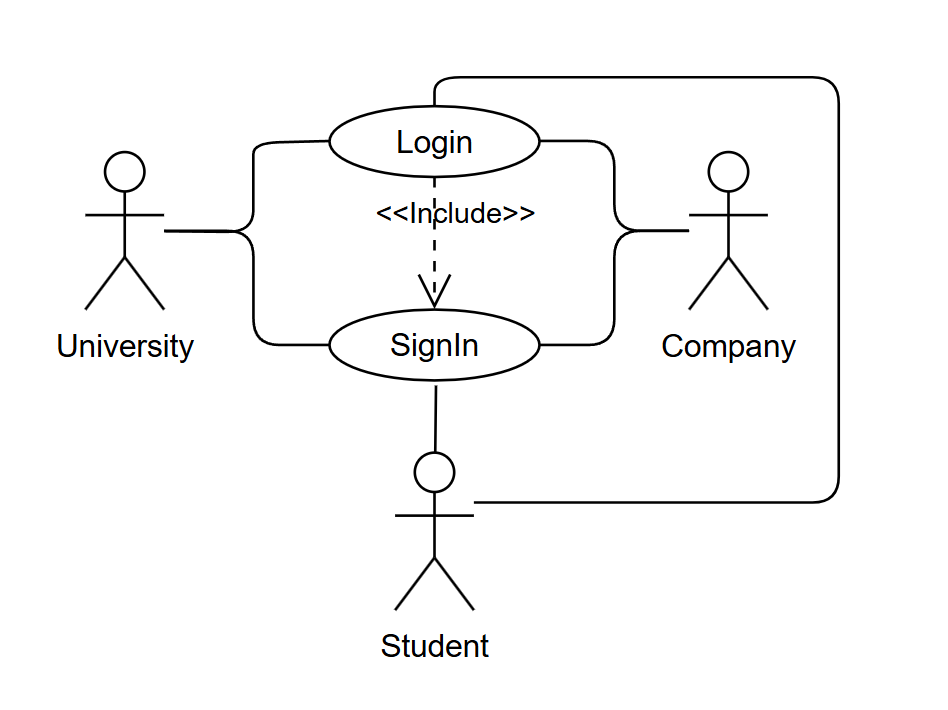
\includegraphics[width=0.5\linewidth]{Login-Signin.png}
    \caption{SignIn and Login UseCase Diagram}
    \label{fig:enter-label}
\end{figure}
This diagram describe the use case that rapresent the creation profile and the login "al" profile, and this use case is mandatory for all the use cases that follows. In the following subsection there will be more detail on this.

\begin{figure}[H]
    \centering
    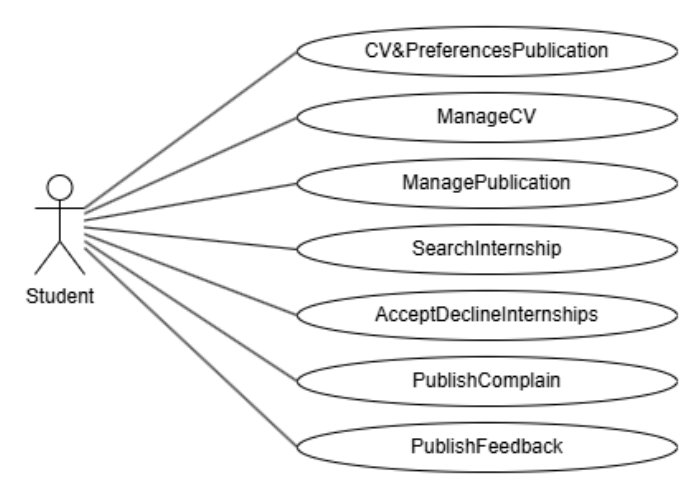
\includegraphics[width=0.5\linewidth]{usecasesStudent.png}
    \caption{Student UseCase Diagram}
    \label{fig:enter-label}
\end{figure}
This diagram describe the student use cases inside S\&C. In the following subsection there will be more detail on this.

\begin{figure}[H]
    \centering
    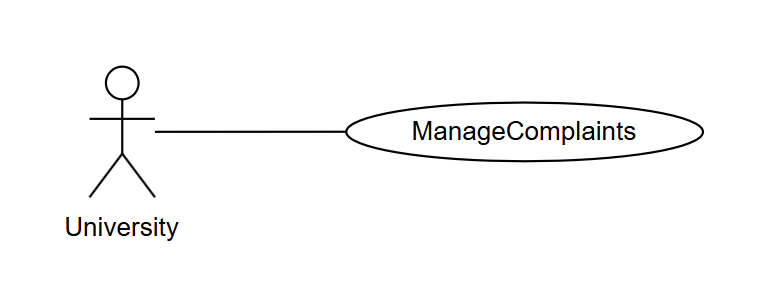
\includegraphics[width=0.5\linewidth]{UniversityUseCases.png}
    \caption{University UseCase Diagram}
    \label{fig:enter-label}
\end{figure}
This diagram describe the university use cases inside S\&C. In the following subsection there will be more detail on this.

\begin{figure}[H]
    \centering
    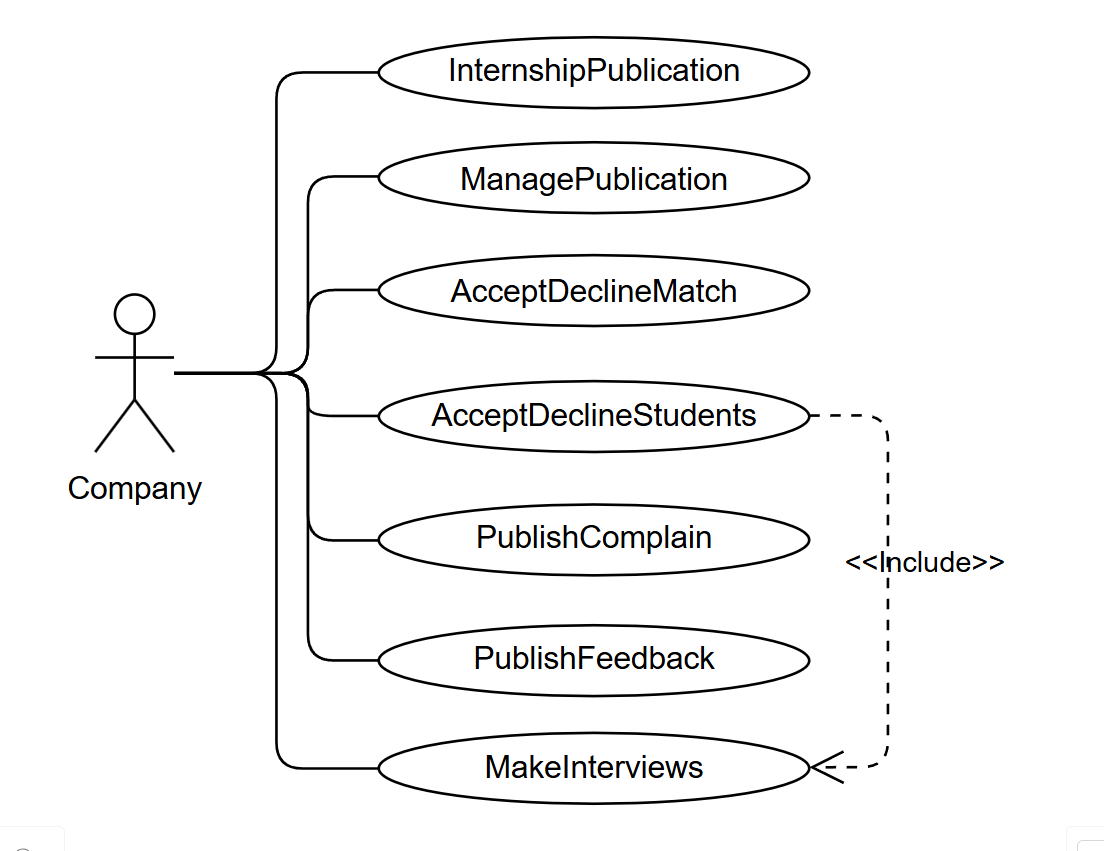
\includegraphics[width=0.5\linewidth]{CompanyUseCases.png}
    \caption{Company UseCase Diagram}
    \label{fig:enter-label}
\end{figure}
This diagram describe the company use cases inside S\&C. In the following subsection there will be more detail on this.

\subsubsection{Use Cases Description}
\textbf{[UC1] SignIn}

\begin{table}[H]
    \centering
    \begin{tabular}{|c|p{10cm}|}
    \hline
        Actor(s)  & User\\ 
    \hline
        Entry Condition &  
        The user accesses the platform and click the signIn button\\
    \hline
        Event Flow &
        \begin{enumerate}
            \item The user visualizes the registration form
\begin{figure}
                \centering
                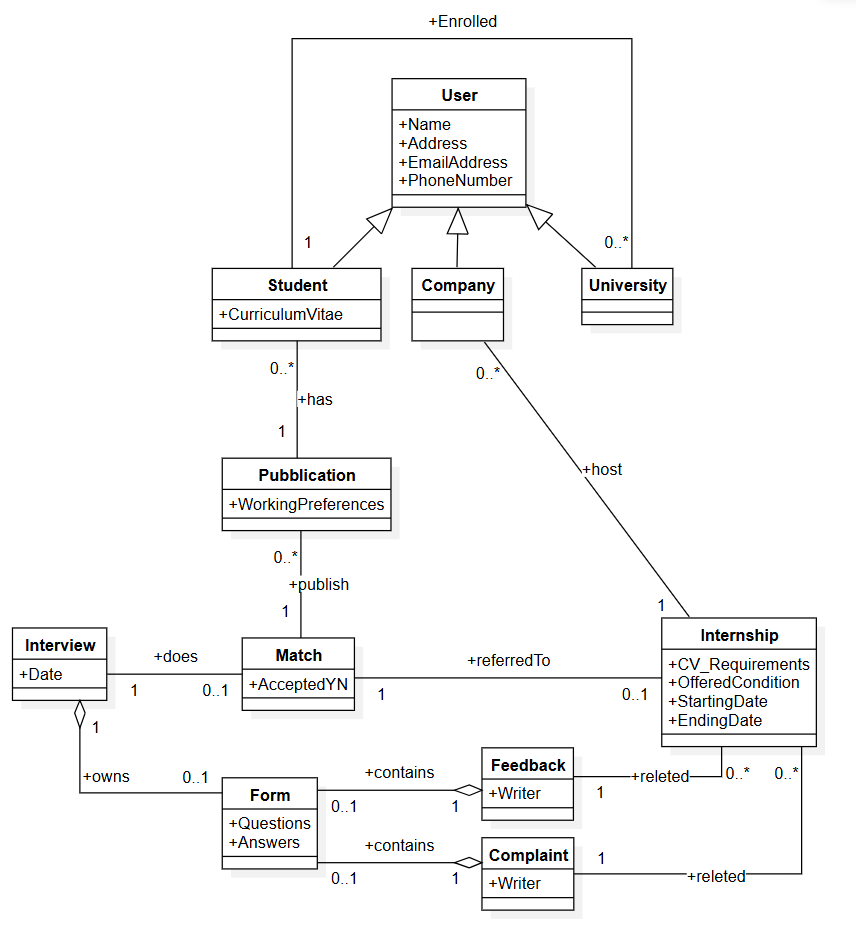
\includegraphics[width=0.5\linewidth]{ClassDiagram.png}
                \caption{Class Diagram}
                \label{fig:enter-label}
\end{figure}
                \item The user fill-in the registration form (name,surname and CV if needed, phone-number, address,email,password)
            \item The user click on the send button, sending the registration form
        \end{enumerate}
        \\
    \hline
        Exit Condition & The user is registered and can access the platform \\
    \hline
        Exceptions &  If provided information is incomplete or invalid, the system prompts the user to correct errors with a human readable message.\\
    \hline
    \end{tabular}
    \label{tab:my_label}
\end{table}
\begin{figure}[H]
    \centering
    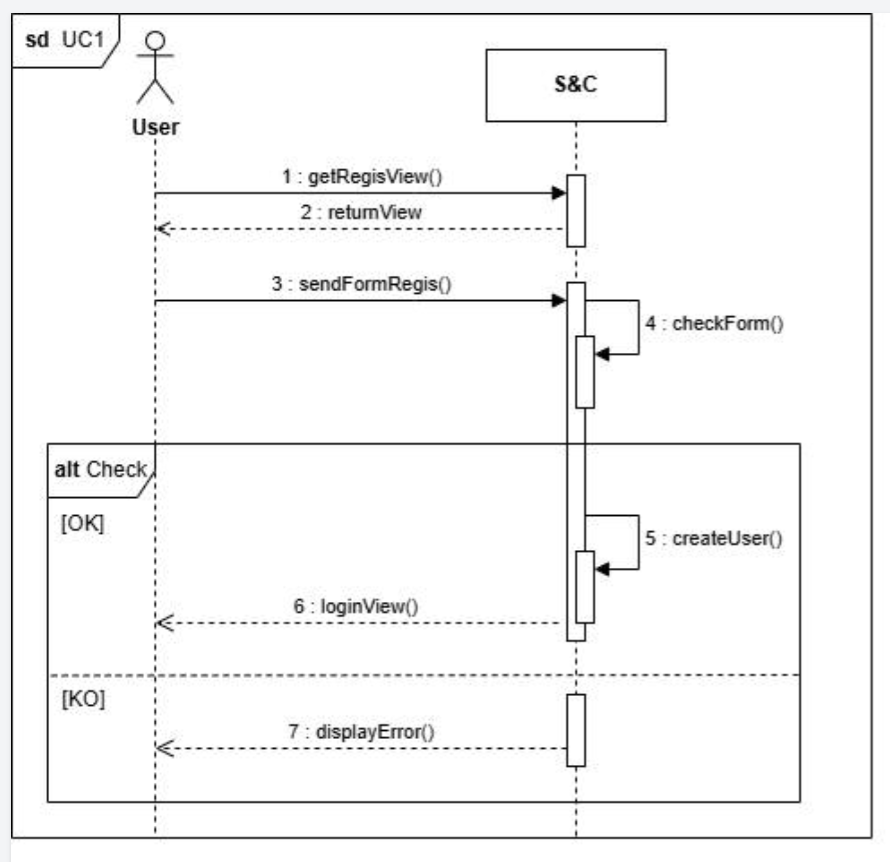
\includegraphics[width=0.8\linewidth]{sequenceDiagrams/UC1.png}
    \caption{"Registration" Sequence Diagram}
    \label{fig:enter-label}
\end{figure}

\vspace{1cm}
\textbf{[UC2] Login}

\begin{table}[H]
    \centering
    \begin{tabular}{|c|p{10cm}|}
    \hline
        Actor(s)  & User\\ 
    \hline
        Entry Condition &  
        The user accesses the platform and has already created an account\\
    \hline
        Event Flow &
        \begin{enumerate}
            \item The user visualizes the login form
            \item The user fill-in the login form (email,password)
            \item The user click on the enter button, entering in the platform
        \end{enumerate}
        \\
    \hline
        Exit Condition & The user has accessed to the platform and can, now, navigate inside the platform\\
    \hline
        Exceptions &  If provided information is incomplete or invalid, the system prompts the user to correct errors with a human readable message.\\
    \hline
    \end{tabular}
    \label{tab:my_label}
\end{table}
\begin{figure}[H]
    \centering
    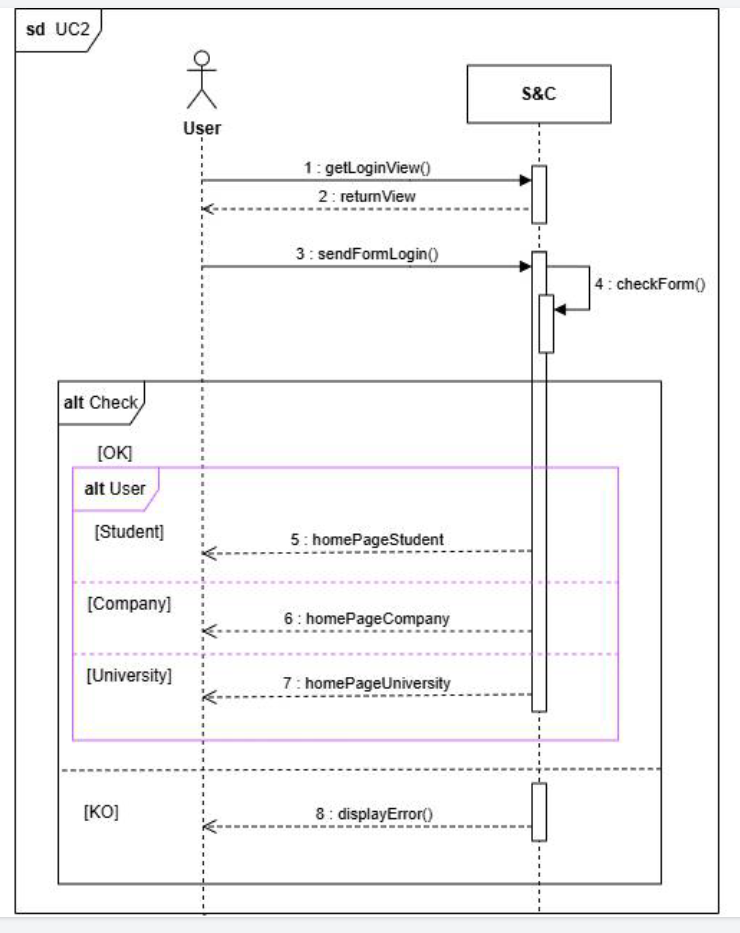
\includegraphics[width=0.8\linewidth]{sequenceDiagrams/UC2.png}
    \caption{"Login" Sequence Diagram}
    \label{fig:enter-label}
\end{figure}
\textbf{STUDENT}\newline\newline
\textbf{[UC3] CV\&PreferencesPublication}

\begin{table}[H]
    \centering
    \begin{tabular}{|c|p{10cm}|}
    \hline
        Actor(s)  & Student\\ 
    \hline
        Entry Condition &  
        The student has logged in the platform \\
    \hline
        Event Flow &
        \begin{enumerate}
            \item The user clicks the button that allows him to publish his internship search announcement
            \item The user insert his CV and send it to the server, which elaborates and sends back the suggestions. Then the student can modify and confirm the updated cv or the previous one. Later, the student enters their internship preferences description.
            \item The user clicks the button to publish the announcement.
            \item The system publishes the announcement and redirects the user to the homepage, then it starts the matchmaking.
        \end{enumerate}
         \\
    \hline
        Exit Condition & The user has published the announce and has returned to the homepage \\
    \hline
        Exceptions &  If provided information is incomplete, the system prompts the user to add the missing informations with a human readable message.\\
    \hline
    \end{tabular}
    \label{tab:my_label}
\end{table}
\begin{figure}[H]
    \centering
    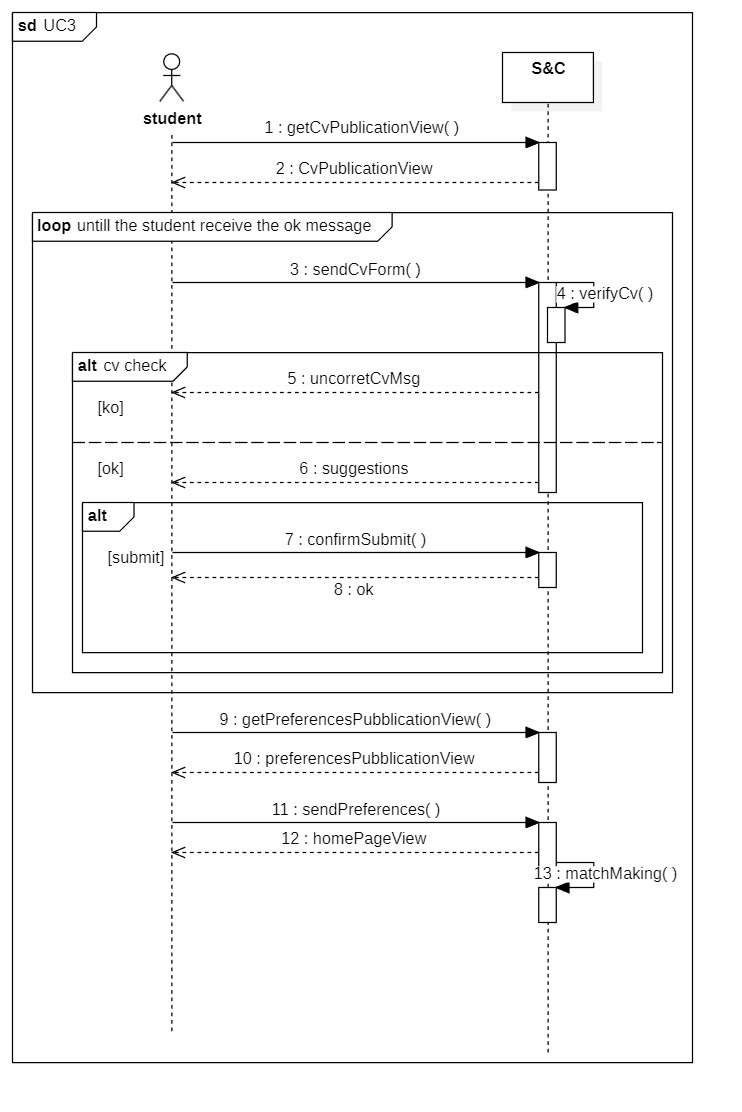
\includegraphics[width=1\linewidth]{sequenceDiagrams/UC3.jpg}
    \caption{"CV\&PublicationPrefernces" Sequence Diagram}
\end{figure}
\textbf{[UC4] ManageCV}

\begin{table}[H]
    \centering
    \begin{tabular}{|c|p{10cm}|}
    \hline
        Actor(s)  & Student\\ 
    \hline 
        Entry Condition &          
        The student has logged in the platform and has added an announce \\
    \hline
        Event Flow &
        \begin{enumerate}
            \item The user clicks the button that allows them to modify their CV
            \item The user modifies, updates (with system's suggestions) or deletes their CV
            \item The user clicks the button to confirm or cancel the changes just made
            \item The system updates their data in order to have right information for the matching 
            \item The system redirects the Student to the homepage
        \end{enumerate}
         \\
    \hline
        Exit Condition & The user has published the modified CV and has returned to the homepage \\
    \hline
        Exceptions &  If provided information is incomplete, the system prompts the user to add the missing informations with a human readable message.\\
    \hline
    \end{tabular}
    \label{tab:my_label}
\end{table}
\begin{figure}[H]
    \centering
    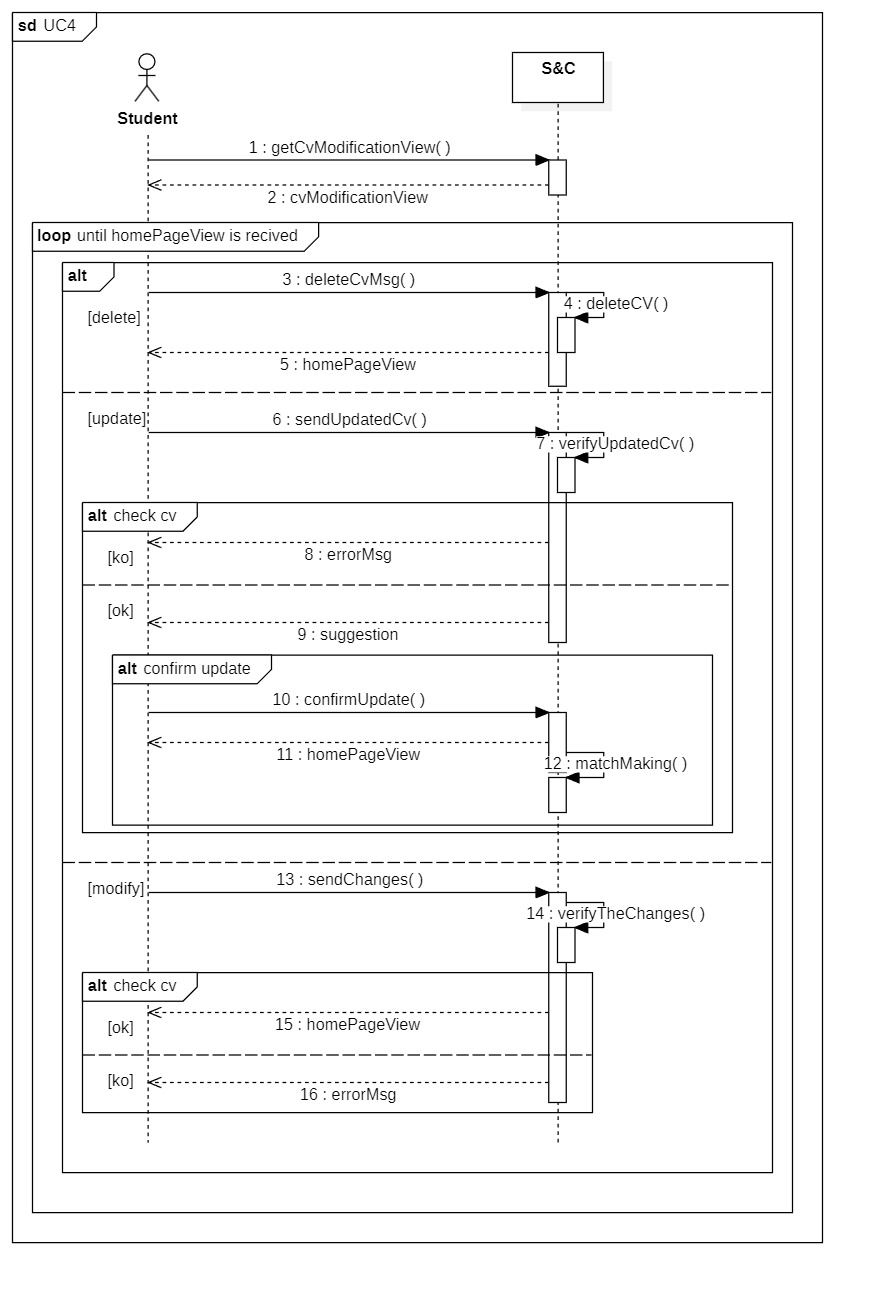
\includegraphics[width=1\linewidth]{sequenceDiagrams/UC4.jpg}
    \caption{"ManageCV” Sequence Diagram}
    \label{fig:enter-label}
\end{figure}
\vspace{1cm}
\textbf{[UC5] ManagePublication}

\begin{table}[H]
    \centering
    \begin{tabular}{|c|p{10cm}|}
    \hline
        Actor(s)  & Student\\ 
    \hline
        Entry Condition &  
        The student has logged in the platform and has added an announce\\
    \hline
        Event Flow &
        \begin{enumerate}
            \item The user click the button that allow him to modify a particular publication 
            \item The user modify or delete that publication
            \item The user click the button to confirm or cancel the changes just made
            \item The system update his data in order to have right information for the matching
            \item The system redirect the Student to the homepage and then start the match making.
        \end{enumerate}
        \\
    \hline
        Exit Condition & The user has modified the publication and return to the homepage\\
    \hline
        Exceptions &  None\\
    \hline
    \end{tabular}
    \label{tab:my_label}
\end{table}
\begin{figure}[H]
    \centering
    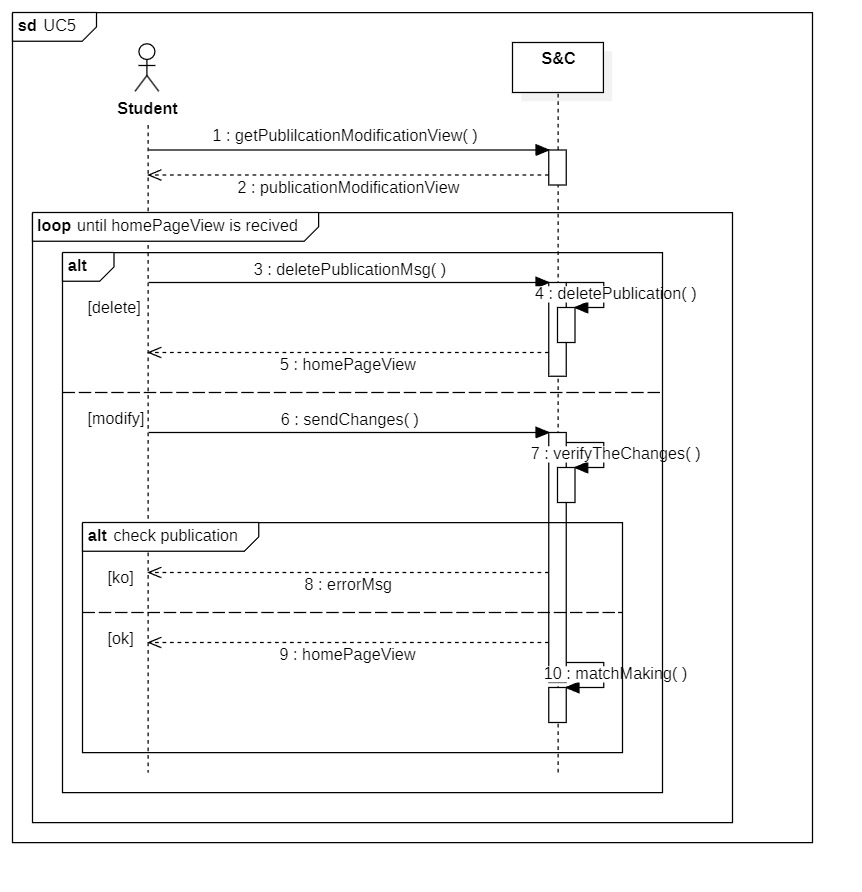
\includegraphics[width=1\linewidth]{sequenceDiagrams/UC5.jpg}
    \caption{"ManagePubblications” Sequence Diagram}
    \label{fig:enter-label}
\end{figure}
\vspace{1cm}
\textbf{[UC6] Search Internship}

\begin{table}[H]
    \centering
    \begin{tabular}{|c|p{10cm}|}
    \hline
        Actor(s)  & Student, Company\\ 
    \hline
        Entry Condition &  
        The student has logged in the platform and has added an announce\\
    \hline
        Event Flow &
        \begin{enumerate}
            \item The user scrolls the homepage and find an interesting internship
            \item The user clicks the button to apply for that internship
            \item The system sends a notification to the corresponding Company to let it know about the new match found
            \item The system redirects the Student to the homepage
        \end{enumerate}
        \\
    \hline
        Exit Condition & The user has made an application and is now in the homepage\\
    \hline
        Exceptions &  None\\
    \hline
    \end{tabular}
    \label{tab:my_label}
\end{table}
\begin{figure}[H]
    \centering
    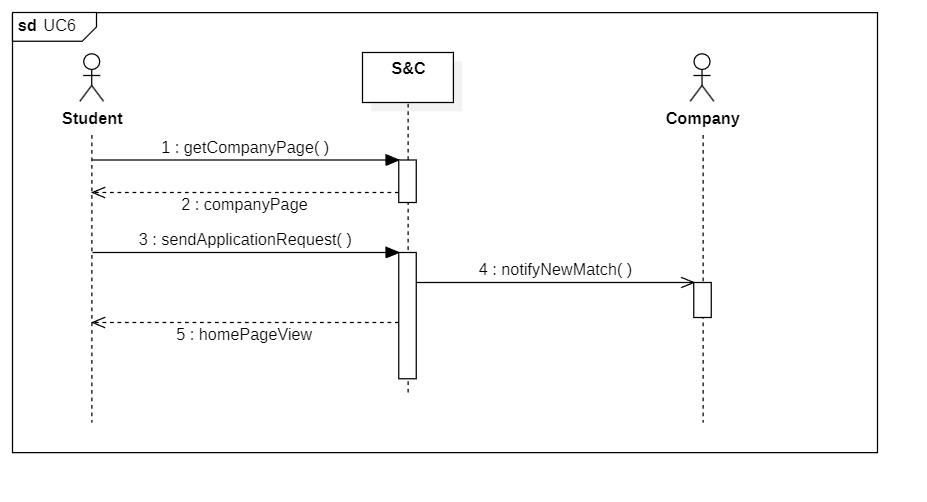
\includegraphics[width=1\linewidth]{sequenceDiagrams/UC6.jpg}
    \caption{"SearchInternships” Sequence Diagram}
    \label{fig:enter-label}
\end{figure}
\vspace{1cm}
\textbf{[UC7] AcceptDeclineInternships}

\begin{table}[H]
    \centering
    \begin{tabular}{|c|p{10cm}|}
    \hline
        Actor(s)  & Student, Company\\ 
    \hline
        Entry Condition &  
        The student has logged in the platform and has added an announce\\
    \hline
        Event Flow &
        \begin{enumerate}
            \item The student receives a notification about a new match found  (optional)
            \item The student goes to the section where he can view all the matches found (optional)
            \item The student clicks on a match found 
            \item the student selects a match
            \item The student clicks the button to accept or decline a particular match
            \item The system sends a notification to the corresponding Company to let it know about the Student's decision
        \end{enumerate}
        \\
    \hline
        Exit Condition & The user has accepted or declined a match\\
    \hline
        Exceptions &  None\\
    \hline
    \end{tabular}
    \label{tab:my_label}
\end{table}
\begin{figure}[H]
    \centering
    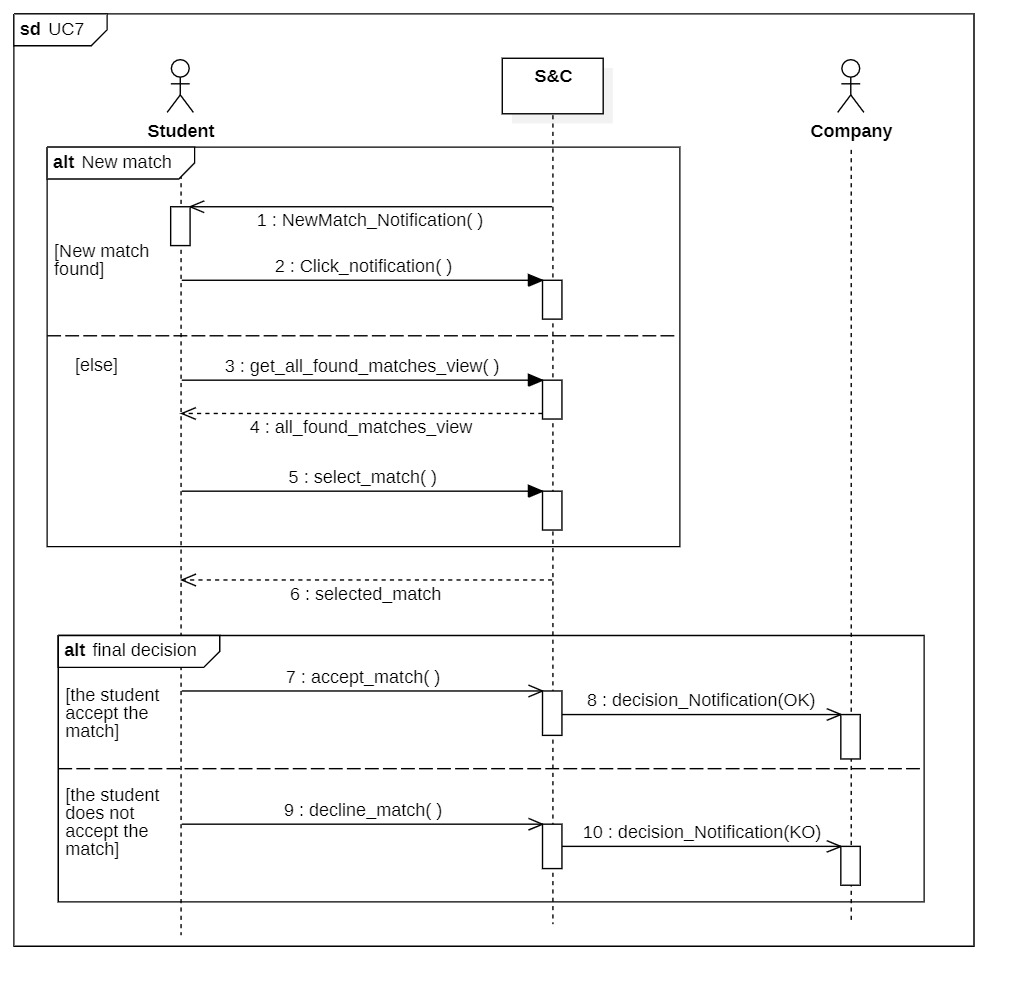
\includegraphics[width=1\linewidth]{sequenceDiagrams/UC7.jpg}
    \caption{"AcceptDeclineInternships” Sequence Diagram}
    \label{fig:enter-label}
\end{figure}

\vspace{1cm}
\textbf{[UC8] PublishComplain}

\begin{table}[H]
    \centering
    \begin{tabular}{|c|p{10cm}|}
    \hline
        Actor(s)  & Student, University\\ 
    \hline
        Entry Condition &  
        The student has logged in the platform and has an ongoing internship\\
    \hline
        Event Flow &
        \begin{enumerate}
            \item The user goes to the section where he can view his internship
            \item The user click the button to create a complain
            \item The user write the complain
            \item The user click the confirm or cancel the complain
            \item The system send a notification to his University to let it know about the Student's complain
            \item The system redirect the Student to the homepage
        \end{enumerate}
        \\
    \hline
        Exit Condition & The user has uploaded the complain\\
    \hline
        Exceptions &  If the text written is empty, the system prompts the Student to add a text with a human readable message.\\
    \hline
    \end{tabular}
    \label{tab:my_label}
\end{table}
\begin{figure}[H]
    \centering
    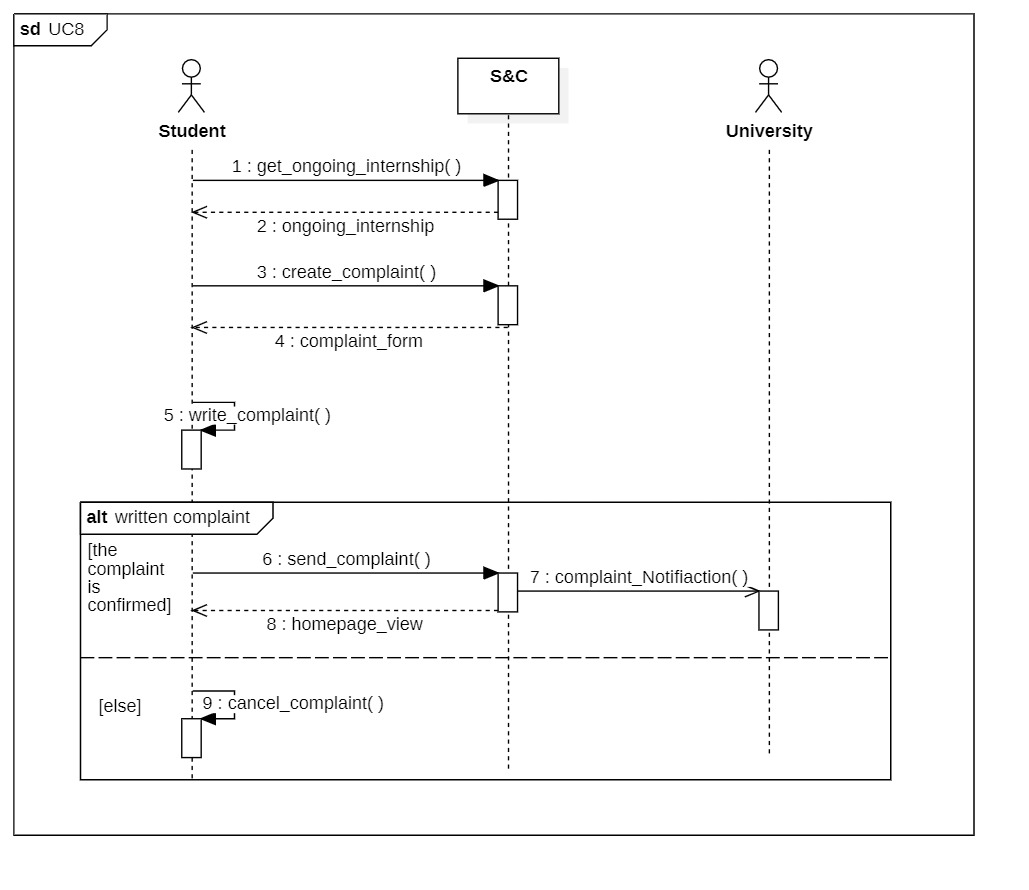
\includegraphics[width=1\linewidth]{sequenceDiagrams/UC8.jpg}
    \caption{"PublishComplain” Sequence Diagram}
    \label{fig:enter-label}
\end{figure}
\vspace{1cm}
\textbf{[UC9] PublishFeedback}

\begin{table}[H]
    \centering
    \begin{tabular}{|c|p{10cm}|}
    \hline
        Actor(s)  & Student, Company\\ 
    \hline
        Entry Condition &  
        The student has logged in the platform and has finished an internship\\
    \hline
        Event Flow &
        \begin{enumerate}
            \item The user receive a notification from the system to write a feedback about the internship just finished
            \item The user click the button to write the feedback
            \item The user write the feedback
            \item The user click the button to confirm the feedback
            \item The system collects the feedback 
            \item The system redirect the Student to the homepage
        \end{enumerate}
        \\
    \hline
        Exit Condition & The user has uploaded the feedback\\
    \hline
        Exceptions &  If the text written is empty, the system prompts the Student to add a text with a human readable message.\\
    \hline
    \end{tabular}
    \label{tab:my_label}
\end{table}
\begin{figure}[H]
    \centering
    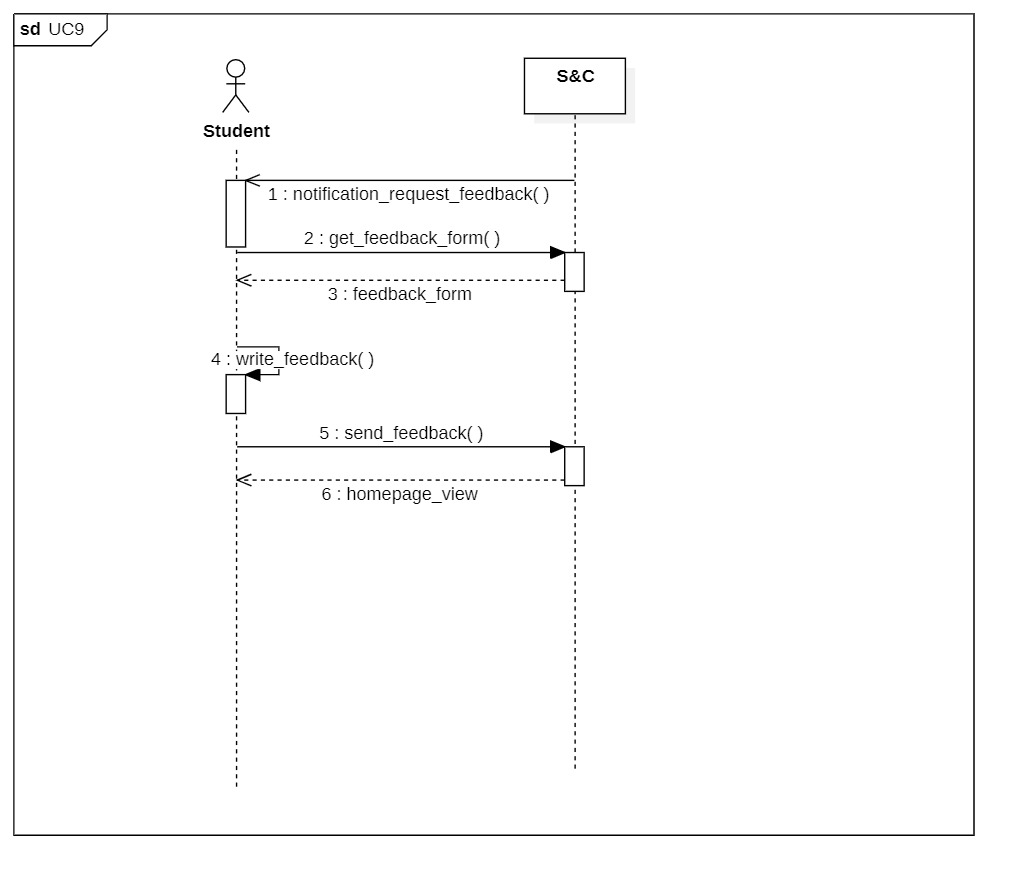
\includegraphics[width=1\linewidth]{sequenceDiagrams/UC9.jpg}
    \caption{"PublishFeedback” Sequence Diagram}
    \label{fig:enter-label}
\end{figure}

\textbf{UNIVERSITY}\newline\newline
\vspace{1cm}
\textbf{[UC10] ManageComplains}

\begin{table}[H]
    \centering
    \begin{tabular}{|c|p{10cm}|}
    \hline
        Actor(s)  & University\\ 
    \hline
        Entry Condition &  
        The university has logged in the platform and has at least one student
        subscribed too\\
    \hline
        Event Flow &
        \begin{enumerate}
            \item The university receive a notification from the system about a new complain wrote by one of its students
            \item The university click on the terminate or cancel button deciding if it's better to conclude or not the internship
            \item The system update the correspond data
            \item The system redirect the university to the homepage
        \end{enumerate}
        \\
    \hline
        Exit Condition & The university has chosen what to do\\
    \hline
        Exceptions &  None\\
    \hline
    \end{tabular}
    \label{tab:my_label}
\end{table}
\begin{figure}[H]
    \centering
        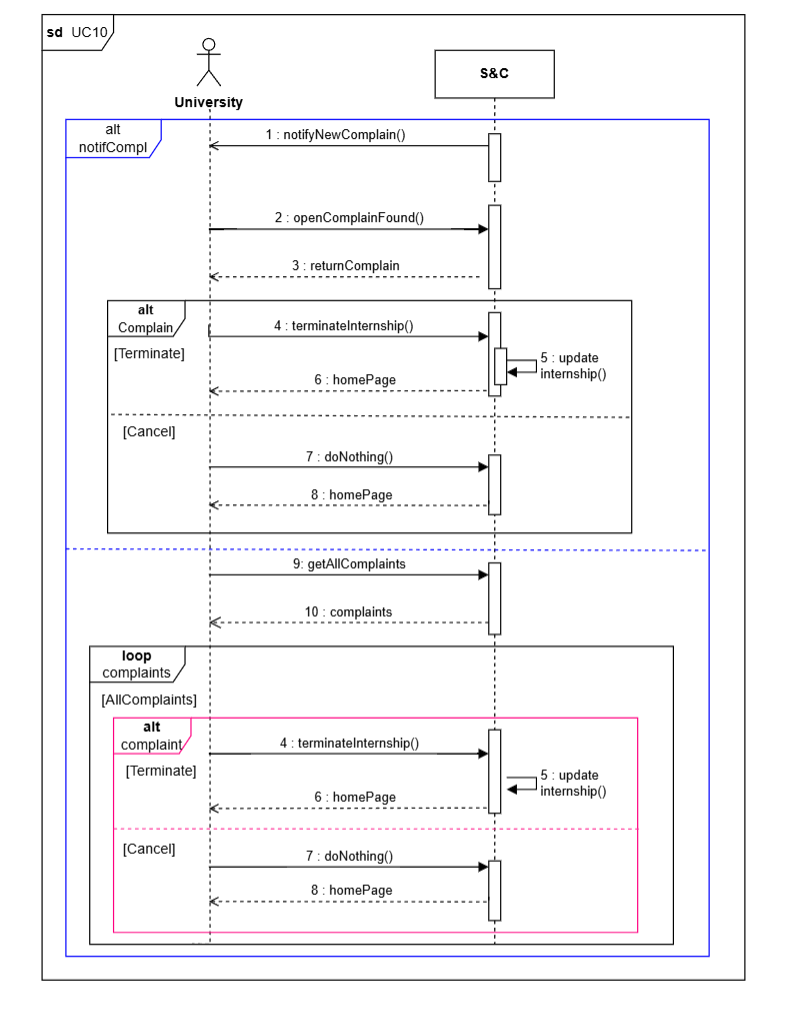
\includegraphics[width=0.8\linewidth]{sequenceDiagrams/UC10.png}
    \caption{"ManageComplains" Sequence Diagram}
    \label{fig:enter-label}
\end{figure}
\textbf{COMPANY}\newline\newline
\vspace{1cm}
\textbf{[UC11] InternshipPublication}

\begin{table}[H]
    \centering
    \begin{tabular}{|c|p{10cm}|}
    \hline
        Actor(s)  & Company\\ 
    \hline
        Entry Condition &  
        The company has logged in the platform \\
    \hline
        Event Flow &
        \begin{enumerate}
            \item The user clicks the button that allows him to publish his announcement regarding the new internship available 
            \item The user inserts the project and submits it to the system, which computes the suggestions and send them back. Then the user can modify the project or confirm the previous version. Finally the the user writes a description about the student's requirements
            \item The user clicks on the button to publish the announcement
            \item The system publishes the announcement and redirects the user to the homepage
        \end{enumerate}
         \\
    \hline
        Exit Condition & The user has published the announce and has returned to the homepage \\
    \hline
        Exceptions &  If provided information is incomplete, the system prompts the user to add the missing informations with a human readable message.\\
    \hline
    \end{tabular}
    \label{tab:my_label}
\end{table}
\begin{figure}[H]
    \centering
    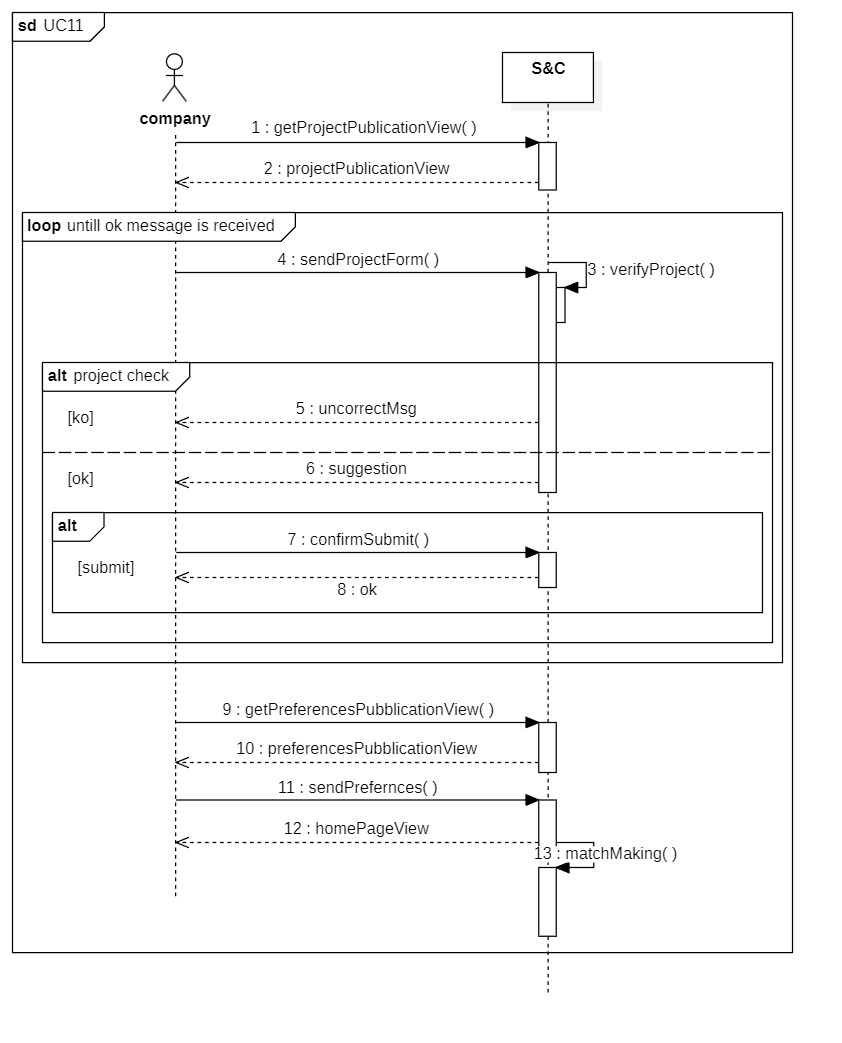
\includegraphics[width=1\linewidth]{sequenceDiagrams/UC11.jpg}
    \caption{"InternshipPublication” Sequence Diagram}
    \label{fig:enter-label}
\end{figure}
\vspace{1cm}
\textbf{[UC12] ManagePublication}

\begin{table}[H]
    \centering
    \begin{tabular}{|c|p{10cm}|}
    \hline
        Actor(s)  & Company\\ 
    \hline
        Entry Condition &  
        The company has logged in the platform and has added an announce\\
    \hline
        Event Flow &
        \begin{enumerate}
            \item The user clicks the button that allows him to modify a particular publication 
            \item The user modifies, updatse (with system’s suggestions) it or deletes that publication, also with the help  the system
            \item The user clicks the button to confirm or cancel the changes just made
            \item The system updates his data in order to have the 
            right information for the matching 
            \item The system redirect the user to the homepage
        \end{enumerate}\\
    \hline
        Exit Condition & The user has modified the publication and return to the homepage\\
    \hline
        Exceptions &  None\\
    \hline
    \end{tabular}
    \label{tab:my_label}
\end{table}

\begin{figure}[H]
    \centering
    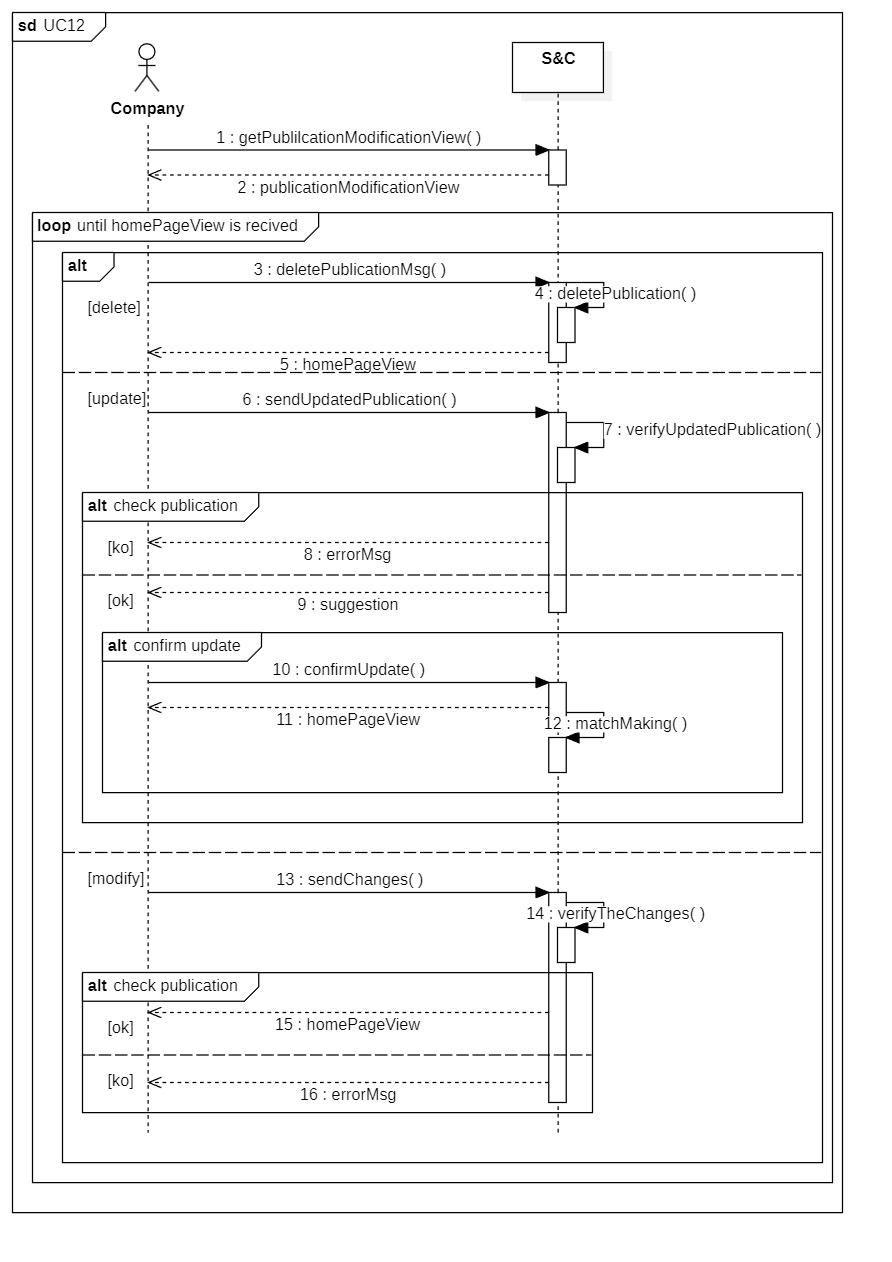
\includegraphics[width=1\linewidth]{sequenceDiagrams/UC12.jpg}
    \caption{"ManagePublication” Sequence Diagram}
    \label{fig:enter-label}
\end{figure}

\vspace{1cm}
\textbf{[UC13] AcceptDeclineMatch}

\begin{table}[H]
    \centering
    \begin{tabular}{|c|p{10cm}|}
    \hline
        Actor(s)  & Company,Student\\ 
    \hline
        Entry Condition &  
        The company has logged in the platform and has added an announce\\
    \hline
        Event Flow &
        \begin{enumerate}
            \item The company receive a notification about a new match found  (optional)
            \item The company goes to the section where it can view all the matches found (optional)
            \item The company click on a match found 
            \item The company click the confirm or cancel button 
            \item The system send a notification to the corresponding Student to let it know about the Company's decision
        \end{enumerate}
        \\
    \hline
        Exit Condition & The company has accepted or declined the student after the match found\\
    \hline
        Exceptions &  None\\
    \hline
    \end{tabular}
    \label{tab:my_label}
\end{table}
\begin{figure}[H]
    \centering
    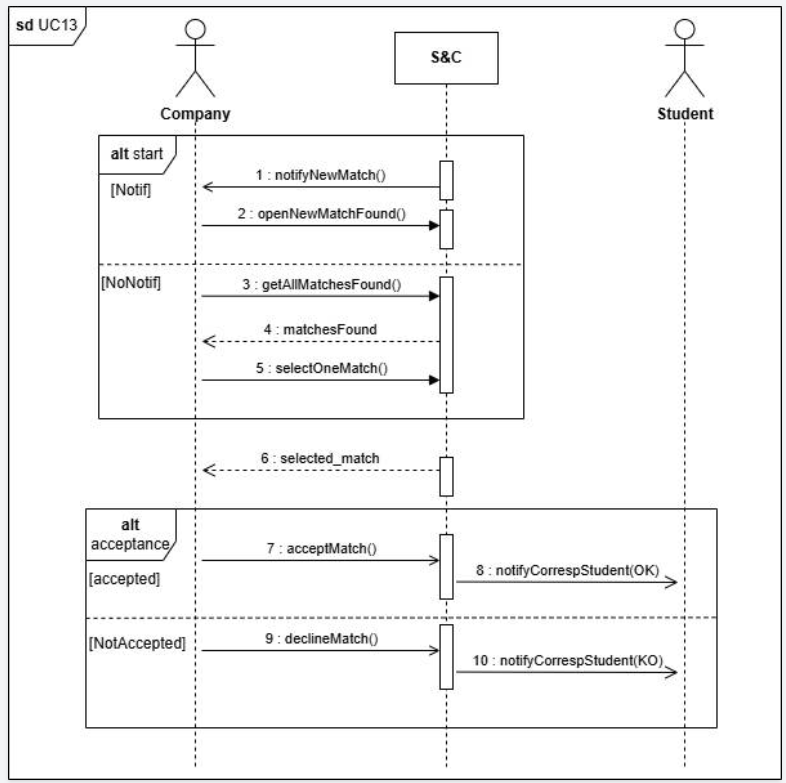
\includegraphics[width=1\linewidth]{sequenceDiagrams/UC13.png}
    \caption{"AcceptDeclineMatch” Sequence Diagram}
    \label{fig:enter-label}
\end{figure}
\vspace{1cm}
\textbf{[UC14] AcceptDeclineStudent}

\begin{table}[H]
    \centering
    \begin{tabular}{|c|p{10cm}|}
    \hline
        Actor(s)  & Company,Student\\ 
    \hline
        Entry Condition &  
        The company has logged in the platform,has added an announce, has accepted a match and created an interview\\
    \hline
        Event Flow &
        \begin{enumerate}
            \item The company goes to the platform's section where all the made interviews are visible
            \item The company select an interview
            \item The company click the accept/decline button 
            \item The system sends a notification to the corresponding Student to let it know about the Company's final decision
        \end{enumerate}
        \\
    \hline
        Exit Condition & The company has accepted or declined the student after the interview\\
    \hline
        Exceptions &  None\\
    \hline
    \end{tabular}
    \label{tab:my_label}
\end{table}
\begin{figure}[H]
    \centering
    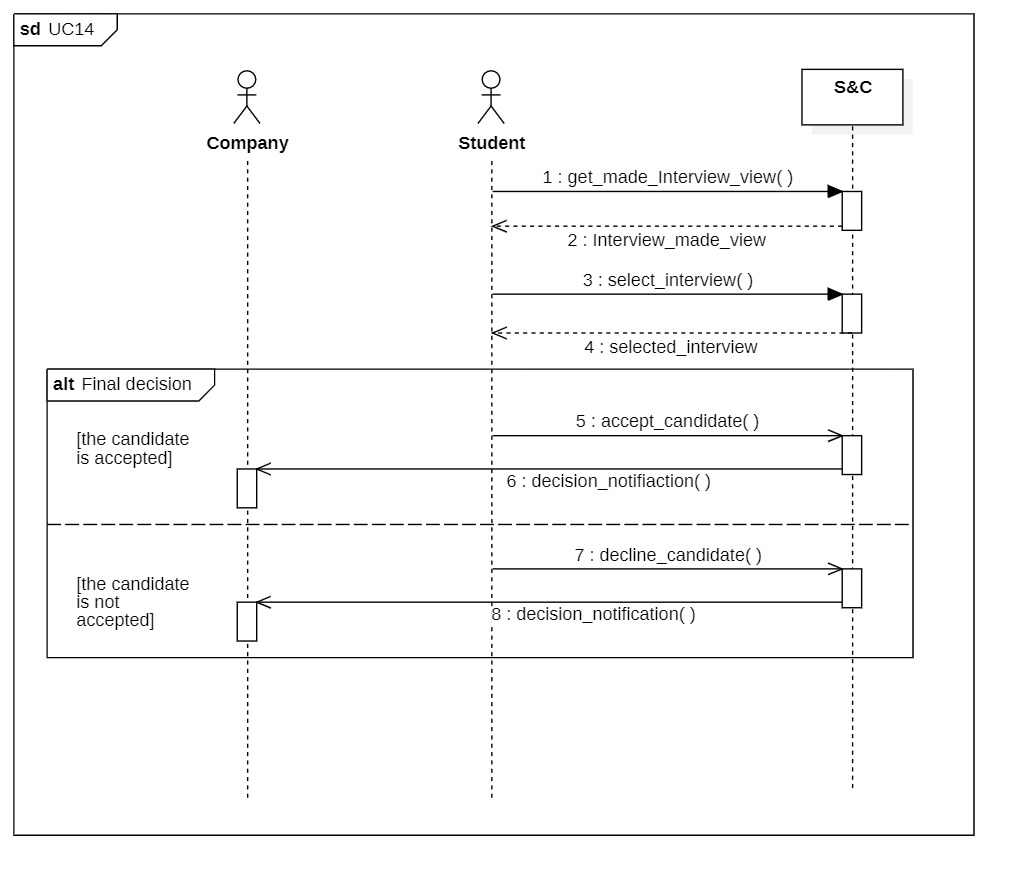
\includegraphics[width=1\linewidth]{sequenceDiagrams/UC14.jpg}
    \caption{"AcceptDeclineStudent” Sequence Diagram}
    \label{fig:enter-label}
\end{figure}
\vspace{1cm}
\textbf{[UC15] PublishComplaint}

\begin{table}[H]
    \centering
    \begin{tabular}{|c|p{10cm}|}
    \hline
        Actor(s)  & Company,University\\ 
    \hline
        Entry Condition &  
        The company has logged in the platform and has an ongoing internship\\
    \hline
        Event Flow &
        \begin{enumerate}
            \item The company goes to the section where it can view his ongoing internships
            \item The company selects the wanted internship
            \item The company clicks the button to create a complain
            \item The company writes the complain
            \item The company confirm or cancel the complain
            \item The system sends a notification to the student's university to inform them about the company's complaint regarding the internship.
            \item The system redirect the Company to the homepage
        \end{enumerate}
        \\
    \hline
        Exit Condition & The user has uploaded the complain\\
    \hline
        Exceptions &  If the text written is empty, the system prompts the Student to add a text with a human readable message.\\
    \hline
    \end{tabular}
    \label{tab:my_label}
\end{table}
\begin{figure}[H]
    \centering
    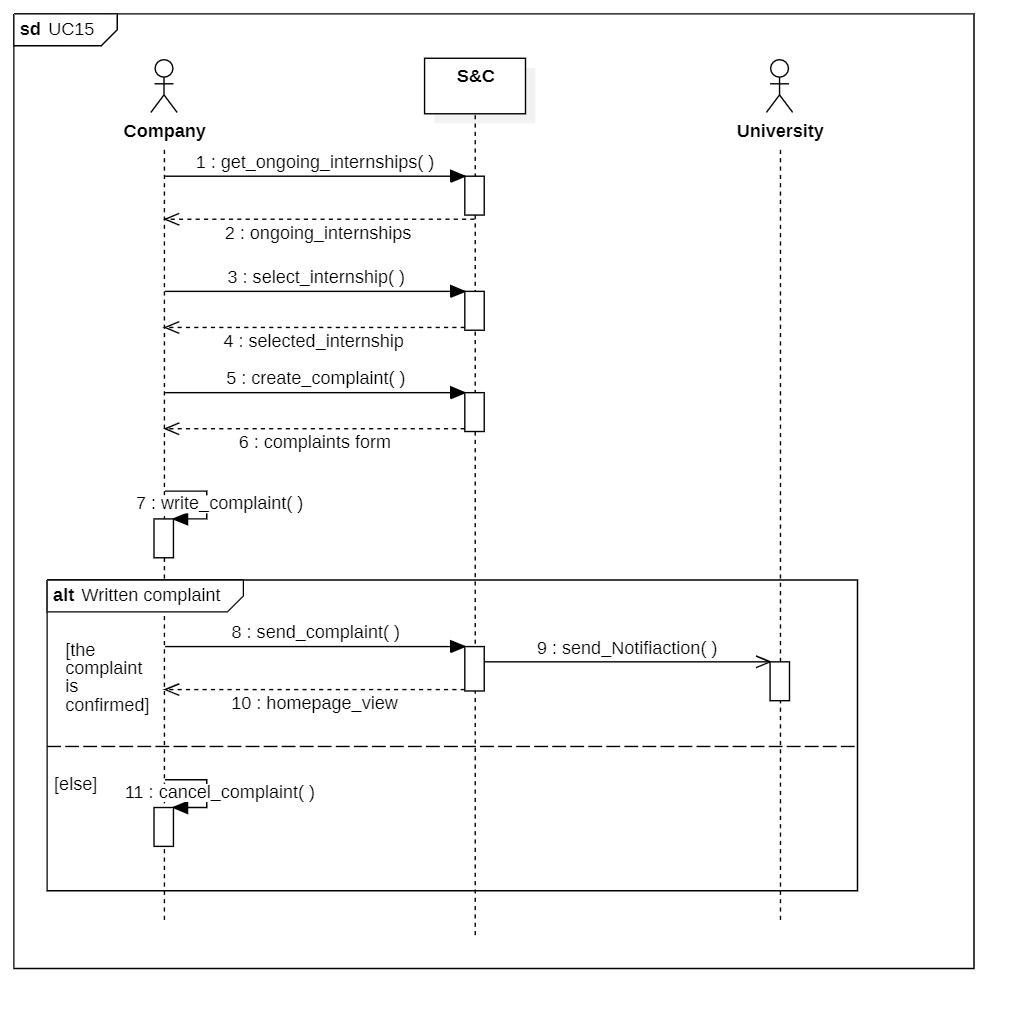
\includegraphics[width=1\linewidth]{sequenceDiagrams/UC15.jpg}
    \caption{"PublishComplain” Sequence Diagram}
    \label{fig:enter-label}
\end{figure}

\vspace{1cm}
\textbf{[UC16] PublishFeedback}

\begin{table}[H]
    \centering
    \begin{tabular}{|c|p{10cm}|}
    \hline
        Actor(s)  & Company\\ 
    \hline
        Entry Condition &  
        The Company has logged in the platform and has ended an internship\\
    \hline
        Event Flow &
        \begin{enumerate}
            \item The company receives a notification from the system to write a feedback about the internship just ended
            \item The company clicks the button to write the feedback
            \item The company writes the feedback
            \item The company clicks the button to confirm the feedback
            \item The system collects the feedback 
            \item The system redirects the company to the homepage
        \end{enumerate}
        \\
    \hline
        Exit Condition & The user has uploaded the feedback\\
    \hline
        Exceptions &  If the text written is empty, the system prompts the Student to add a text with a human readable message.\\
    \hline
    \end{tabular}
    \label{tab:my_label}
\end{table}
\begin{figure}[H]
    \centering
    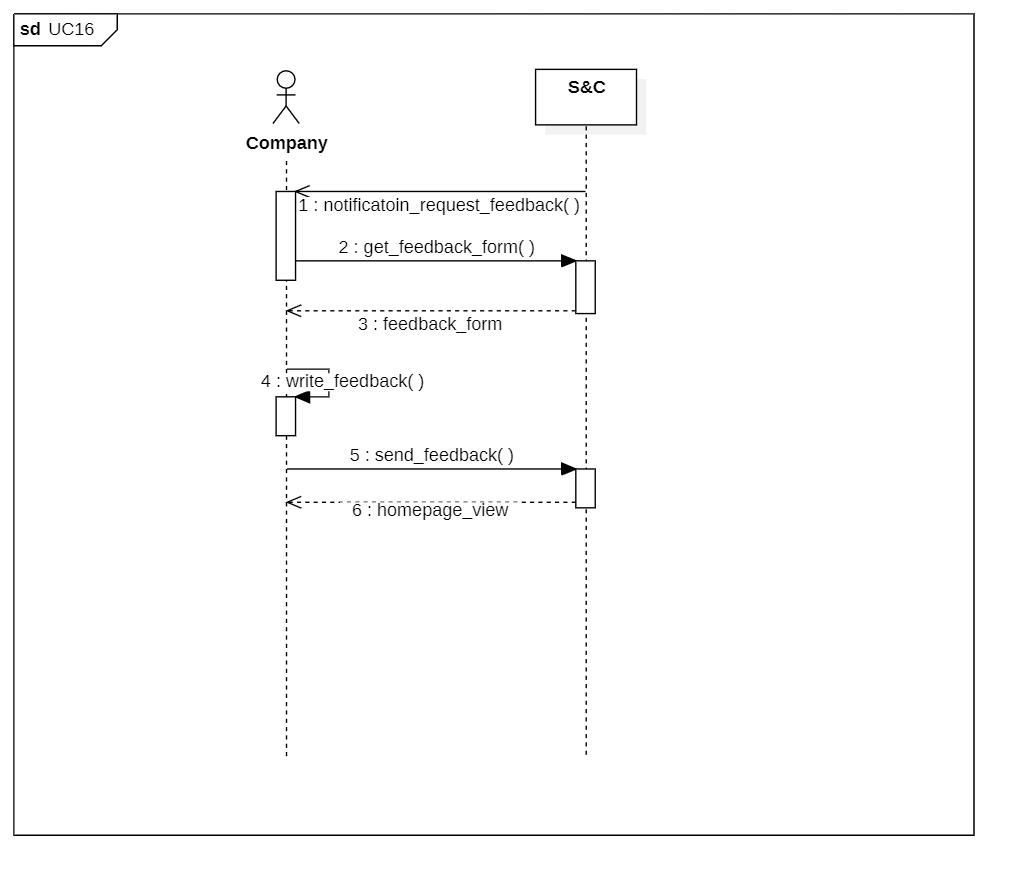
\includegraphics[width=1\linewidth]{sequenceDiagrams/UC16.jpg}
    \caption{"PublishFeedback” Sequence Diagram}
    \label{fig:enter-label}
\end{figure}
\vspace{1cm}
\textbf{[UC17] MakeInterviews}

\begin{table}[H]
    \centering
    \begin{tabular}{|c|p{10cm}|}
    \hline
        Actor(s)  & Company,Student\\ 
    \hline
        Entry Condition &  
        The Company has logged in the platform and has accepted a match\\
    \hline
        Event Flow &
        \begin{enumerate}
            \item The company creates the interview form 
            \item The company fill-in the form with the Student's responses
            \item The company click the button to finish the interview
            \item The system collects the interview 
            \item The system redirect the user to the homepage
        \end{enumerate}
        \\
    \hline
        Exit Condition & The user has uploaded the interview\\
    \hline
        Exceptions &  If the text written is empty, the system prompts the Student to add a text with a human readable message.\\
    \hline
    \end{tabular}
    \label{tab:my_label}
\end{table}
\begin{figure}[H]
    \centering
    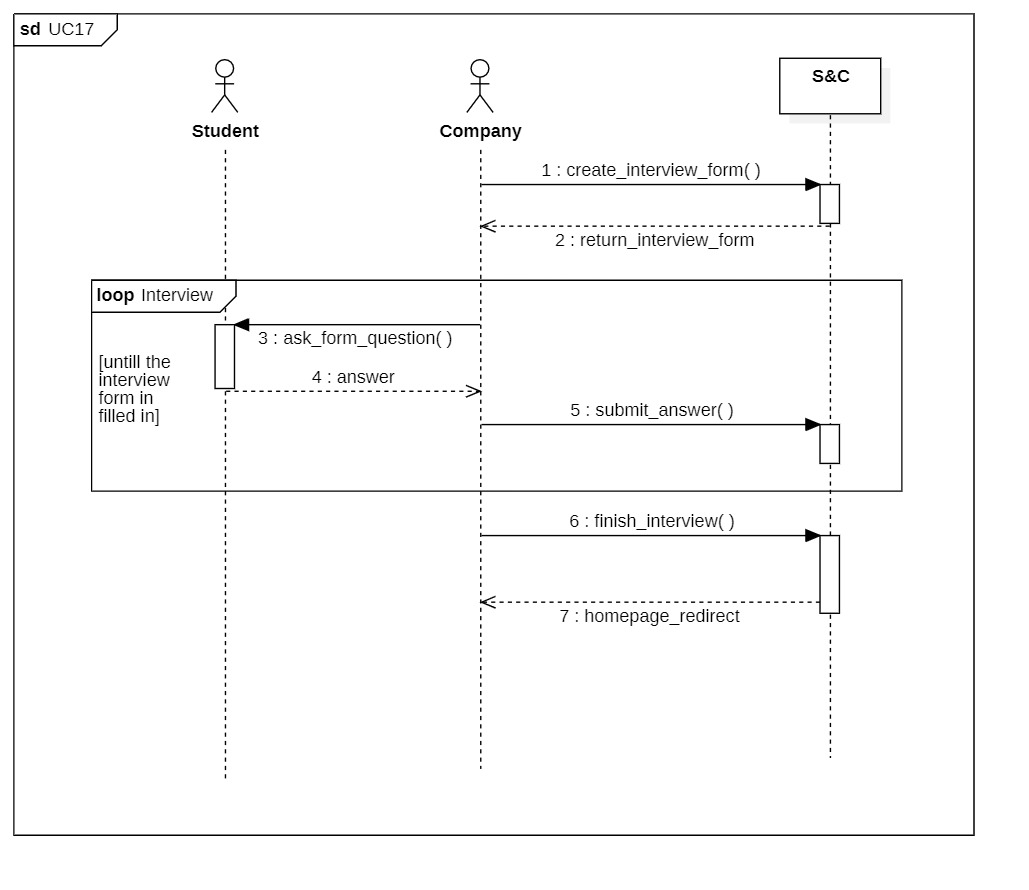
\includegraphics[width=1\linewidth]{sequenceDiagrams/UC17.jpg}
    \caption{"MakeInterview” Sequence Diagram}
    \label{fig:enter-label}
\end{figure}

\subsubsection{Mapping on requirements}

\begin{table}[H]
    \centering
    \begin{tabular}{|p{11cm}|}
        \hline
         G1: Facilitate internship searches for students \\
         \hline
         \textbf{Requirements mapping}\\
         \hline
        [R1] The system shall allow unregistered users to create an account on S\&C only if their university already has an account on the platform.\newline
        [R2] The system shall allow registered users to log in to their accounts.\newline
        [R7] The system shall allow the students to publish their CVs and their preferences delle internship\newline
        [R8] The system shall allow the students to modify their CVs and their preferences delle internship\newline
        [R9] The system shall allow the students to delete their CVs and their preferences delle internship\newline
        [R10] The system shall allow the students to view all the matches found\newline
        [R12] The system shall allow the companies and the students to accept or decline the proposed matches\newline
        [R17] The system shall allow the  students to update their CVs \newline
        [R18] The system shall allow the students to browse through the available internships \newline
        [R19] The system shall allow the students to directly make an application to the available internships \newline
        [R20] The system shall allow the students to send complaints \newline
        [R22] The system shall allow the students to give the final feedback\newline
        [R24] The system shall notify the students whenever a new match is found\newline
        [R27] The system shall suggests students on how to improve their CVs\newline
        [R29] The system shall analyse the students pubblications in order to find a match with the right companies \newline
        [R31] The system shall create matches using different level of sophistication, from simple keyword-search to statistical analyses based final feedbacks made by students and companies \newline\\
         \hline
         \textbf{Domain assumption mapping}\\
         \hline
         [D5] Students and companies must have an email to communicate. \newline
         [D1] The students have to be at the end of their career\newline
         [D2] The CVs have to contain real data\newline
         [D4] The student must have uploaded their CV in EU format to ensure the proper functioning of the application. \newline
         [D6] The student's email must be a university email \newline\\
         \hline
    \end{tabular}
    \caption{Mapping on first goal}
    \label{tab:my_label}
\end{table}

\begin{table}[H]
    \centering
    \begin{tabular}{|p{11cm}|}
        \hline
         G2: Facilitate student searches for companies\\
         \hline
         \textbf{Requirements mapping}\\
         \hline
        [R1] The system shall allow unregistered users to create an account on S\&C only if their university already has an account on the platform.\newline
        [R2] The system shall allow registered users to log in to their accounts.\newline
        [R4] The system shall allow the companies to publish their internships\newline
        [R5] The system shall allow the companies to modify their internships\newline
        [R6] The system shall allow the companies to delete their internships\newline
        [R11] The system shall allow the companies to view all the matches found\newline
        [R12] The system shall allow the companies and the students to accept or decline the proposed matches\newline
        [R21] The system shall allow the companies to send complaints\newline
        [R23] The system shall allow the companies to give the final feedback\newline
        [R26]The system shall notify the companies whenever a new match is found\newline
        [R28] The system shall suggest companies on how to improve their internships proposal\newline
        [R30] The system shall analyse the companies pubblications in order to find a match with the right students \newline
        [R31] The system shall create matches using different level of sophistication, from simple keyword-search to statistical analyses based on final feedbacks made by students and companies \newline\\
         \hline
         \textbf{Domain assumption mapping}\\
         \hline
         [D5] Students and companies must have an email to communicate. \newline
         [D3] The companies have to public only available internship\newline\\
         \hline
    \end{tabular}
    \caption{Mapping on second goal}
    \label{tab:my_label}
\end{table}

\begin{table}[H]
    \centering
    \begin{tabular}{|p{11cm}|}
        \hline
         G3: Interviews support\\
         \hline
         \textbf{Requirements mapping}\\
         \hline
        [R13] The system shall allow the companies to create the interview form.\newline
        [R14] The system shall allow the companies to add responses of the students during the interview, to the form.\newline \\
         \hline
         \textbf{Domain assumption mapping}\\
         \hline
         \\
         \hline
    \end{tabular}
    \caption{Mapping on third goal}
    \label{tab:my_label}
\end{table}

\begin{table}[H]
    \centering
    \begin{tabular}{|p{11cm}|}
        \hline
         G4: Monitoring internship progress \\
         \hline
         \textbf{Requirements mapping}\\
         \hline
        [R1] The system shall allow unregistered users to create an account on S\&C only if their university already has an account on the platform.\newline
        [R2] The system shall allow registered users to log in to their accounts.\newline
        [R3] The system shall allow the universities to request an account on the platform.\newline
        [R15] The system shall allow the universities to manage the complaints which involves their students\newline
        [R16] The system shall allow the universities to stop the on going internships involving their students\newline
        [R25] The system shall notify the universities whenever a new complaint involving one of its students is submitted\newline
        [R32] The system shall allow the universities to see their own students and their ongoing internships\newline\\
         \hline
         \textbf{Domain assumption mapping}\\
         \hline
         \\
         \hline
    \end{tabular}
    \caption{Mapping on fourth goal}
    \label{tab:my_label}
\end{table}

\subsection{Performance Requirements}
\textbf{Number of concurrent Users}: WebApps with a similar goal of S\&C, has million of Users. To guarantee this, means S\&C should be able to handle up at least 10.000 Users simultaneously. This is important for making sure our WebApp works well for a good number of people, giving them a smooth and enjoyable experience.\newline
\textbf{Data storage}: S\&C needs to save and manage all the details about Students, Universities and Companies. Additionally, the database needs to process queries in an efficient way in order to allow user to view all the information they need in short time.\newline
\textbf{Time response}: Every operation that is directly executed by S\&C, i.e. register, login, create, modify and evaluate, should be in the domain of milliseconds.\newline
\textbf{Resources}: S\&C needs to scale its resources up or down based on demand, utilizing cloud based services and load balancing techniques.

\subsection{Design Constraints}
\subsubsection{Standard compliance}
The application should follow all the specific regulations in matter of digital services such as GDPR and the most recent European Digital Service Act. These regulations guarantee safety and transparency over how user data is handled, how content is managed and how the application works (for example explaining how matches are done)
\subsubsection{Hardware limitations}
Being a webApp, the application should be compatible with a large number of devices, from PCs to smartphones. In order to operate correctly a recent version of one of the most used browser (Chrome, Edge, Firefox, Safari, etc ) is required.
Server-side, the hardware must be chosen in order to effectively store all the current and historical information and to provide a response time < 2 sec even under heavy load.
\subsubsection{Any other constraints}
The development of the application should consider that it will be used by a large number of people, thus it should be structured with usability in mind. For example it should be easy to use, accessible and should support multi-language interface.
Moreover, the entire infrastructure should be designed to be scalable.
Finally the matching system should be ethical. This means that the matching algorithm should be neutral and not only based on the students' expertises and internships characteristics but also on final feedbacks made by students and companies (used for statistical analyses matching).

\subsection{Software System Attributes}

\subsubsection{Reliability}

The MTFB of the S\&C should be at least of 1 month and the MTTB should be at most one hour in order to be  better than the expected below constraint. To achieve this reliability we need to implement the application on a set of replicated server, to be resilient in case of failure. 

\subsubsection{Availability}

The needed availability should be at least the 99.7\% to have one day down in a span of a year, if the above constraint in reliability will be reached the probable availability will be more than 99.8\%

\subsubsection{Security}

The S\&C system has to be implemented over HTTPS to communicate in a secure manner with the central server, with the machine in charge of the communication placed in a DMZ to protect the DB. The system must to be able to avoid the SQL INJECTION, the CSRF and the XSS attacks.

\subsubsection{Maintainability}

The S\&C system should be designed in a modular concept in order to be maintainable and fixed with ease. In this context each part of the software must be available through APIs. It is also needed to keep the documentation up to date and run automated tests after each update or fix.

\subsubsection{Portability}

The system should be designed to work on all the common browser (like edge, Chrome, Safari and Firefox etc.) also on the mobile device (like smartphone and tablet).

\section{Formal Analysis Using Alloy}
\begin{spverbatim}
enum Accepted {Yes, No}

abstract sig User{
}


sig Student extends User{
    uni: one University
}

sig University extends User{
}

sig Company extends User{
    
}

sig Publication{
    student : one Student
}

var sig Match {
    var acceptedYN: one Accepted,
    var pub : one Publication,
    var ref : one Internship
}

sig Internship {
    hosted : one Company,
    var feedbacks : set Feedback,
    var complaints : set Complaint
}

var sig Interview {
    var match : one Match,
    var confirmedYN: one Accepted
}

var sig Complaint {
    var writer : one User
}

var sig Feedback {
    var writer : one User
}


//there is no feedback pointed from more internships
fact {
    always no i1, i2: Internship | some f : Feedback|
        f in i1.feedbacks and f in i2.feedbacks and i1 != i2
}

//there is no complaint pointed from more internships
fact {
    always no i1, i2: Internship | some c : Complaint|
        c in i1.complaints and c in i2.complaints and i1 != i2
}

//all the feedback must have an internship 
fact {
    always all f : Feedback | some i : Internship |
        f in i.feedbacks     
}

//all the complaint must have an internship 
fact {
    always all c : Complaint | some i : Internship |
        c in i.complaints     
}


//check the number of writer
fact{
    always all i : Internship | 
        #i.feedbacks <= 2 and #(i.feedbacks.writer & Student) < 2 and #(i.feedbacks.writer & Company) < 2 and 
        #(i.feedbacks.writer & University) = 0
    
}

//only student and company can write complaints 
fact {
    always all i: Internship |
        #(i.complaints.writer & University) = 0
}

//check that if the feedback is written by a company then the company is the one who host the internship
fact {
    always all i : Internship | no f : Feedback|
        f in i.feedbacks and #(f.writer & Company) > 0 and f.writer != i.hosted
}

//check that if the complaint is written by a company then the company is the one who host the internship
fact {
    always all i : Internship | no c: Complaint|
        c in i.complaints and #(c.writer & Company) > 0 and c.writer != i.hosted
}

//check the students writes feedback only to his own matched internships
fact {
    always all i : Internship | no f : Feedback,  m : Match|
        f in i.feedbacks and #(f.writer & Student) > 0 and m.ref = i and m.pub.student != f.writer
}

//check the students writes complaints only to his own matched internships
fact {
    always all i : Internship | no c : Complaint,  m : Match|
        c in i.complaints and #(c.writer & Student) > 0 and m.ref = i and m.pub.student != c.writer
}

//no feedback of the same internship can have the same writer 

fact {
    always all i : Internship | no f1, f2 : Feedback| 
        f1 in i.feedbacks and f2 in i.feedbacks and f1.writer = f2.writer and f1 != f2
}


//check that there is at most one match between a pair of company and student
fact {
    always all m1 : Match | no m2 : Match |
       m1.ref.hosted = m2.ref.hosted and m1.pub.student = m2.pub.student and m1 != m2
}

//only one match with confirmed interview for internships
fact {
    always no i1, i2: Interview |
        i1.confirmedYN = Yes and i2.confirmedYN = Yes and i1.match.ref = i2.match.ref and i1 != i2
}

//only match with confirmed interview can have feedback

fact {
    always all f: Feedback| some m: Match, i : Interview |
        f in m.ref.feedbacks and i.match = m and i.confirmedYN = Yes 
}


//only match with confirmed interview can have complaints
fact {
    always all c: Complaint| some m: Match, i : Interview |
        c in m.ref.complaints and i.match = m and i.confirmedYN = Yes
}


//every match can have at most one interview
fact {
    always no i1, i2 : Interview|
        i1.match = i2.match and i1 != i2
}

//there can be an interview only if the match is accepted

fact{
    always no m: Match | some i : Interview |
        m.acceptedYN = No and i.match = m 
}



//the match once they are added they can't be deleted
fact {
    always (Match in Match')
}

//the match cant change his attributes
fact{
    always all m : Match|
       (m.acceptedYN = No and after(m.acceptedYN = No ))
      or 
       (m.acceptedYN = Yes and after(m.acceptedYN = Yes ))
    
    always all m : Match| some p: Publication|
        m.pub = p and after(m.pub = p)
    
    always all m : Match| some i: Internship|
        m.ref = i and after(m.ref = i)
}


//the interview once they are added they can't be deleted
fact{
    always (Interview in Interview')
}

//the interview cant change his attributes 
fact{
    always all i : Interview|
      always (i.confirmedYN = No implies historically(i.confirmedYN = No ))
      or 
      always (i.confirmedYN = Yes implies historically(i.confirmedYN = Yes ))
    
    always all i : Interview  | some m: Match|
        i.match = m and after(i.match = m)
    
}

//the Feedback once they are added they can't be deleted
fact {
    always (Feedback in Feedback')
}

//the feedback can't change his attributes 
fact{
    always all f : Feedback  | some u: User|
        f.writer = u and after(f.writer = u)    
}

//the Complaint once they are added they can't be deleted
fact{
    always (Complaint in Complaint')
}

//the Complaint can't change his attributes 
fact{
    always all c : Complaint  | some u: User|
       c.writer = u and after(c.writer = u)    
}

pred show{
    no Match; #Match = 2
    no Interview; no Interview; some Interview
    no Complaint; no Complaint; no Complaint; some Complaint
    no Feedback; no Feedback; no Feedback; some Feedback
}


run show for 4
\end{spverbatim}

\begin{figure}[H]
    \centering
    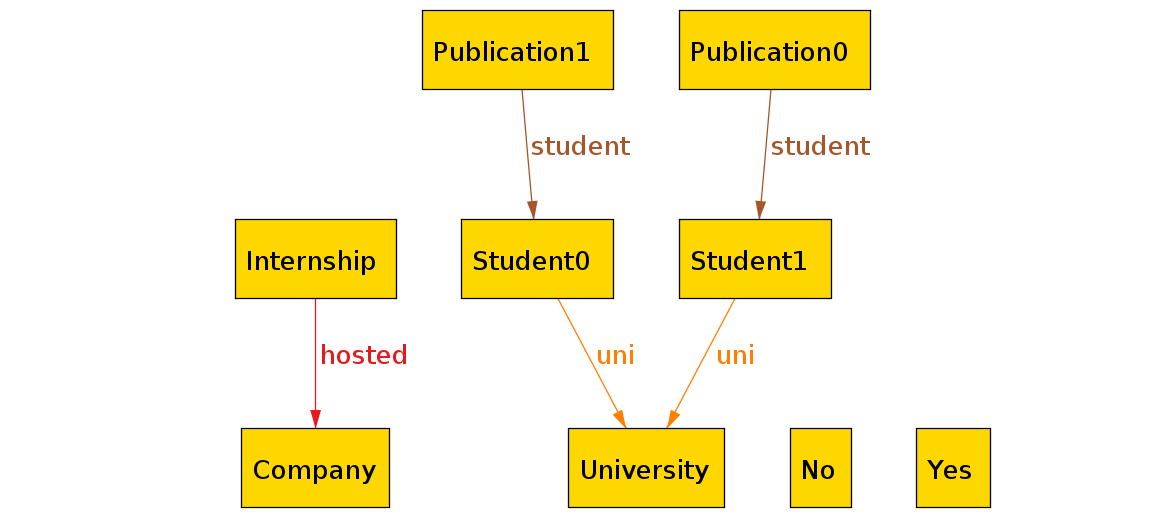
\includegraphics[width=1\linewidth]{alloy/state1.png}
    \caption{Alloy first state}
    \label{fig:state1}
\end{figure}


\begin{figure}[H]
    \centering
    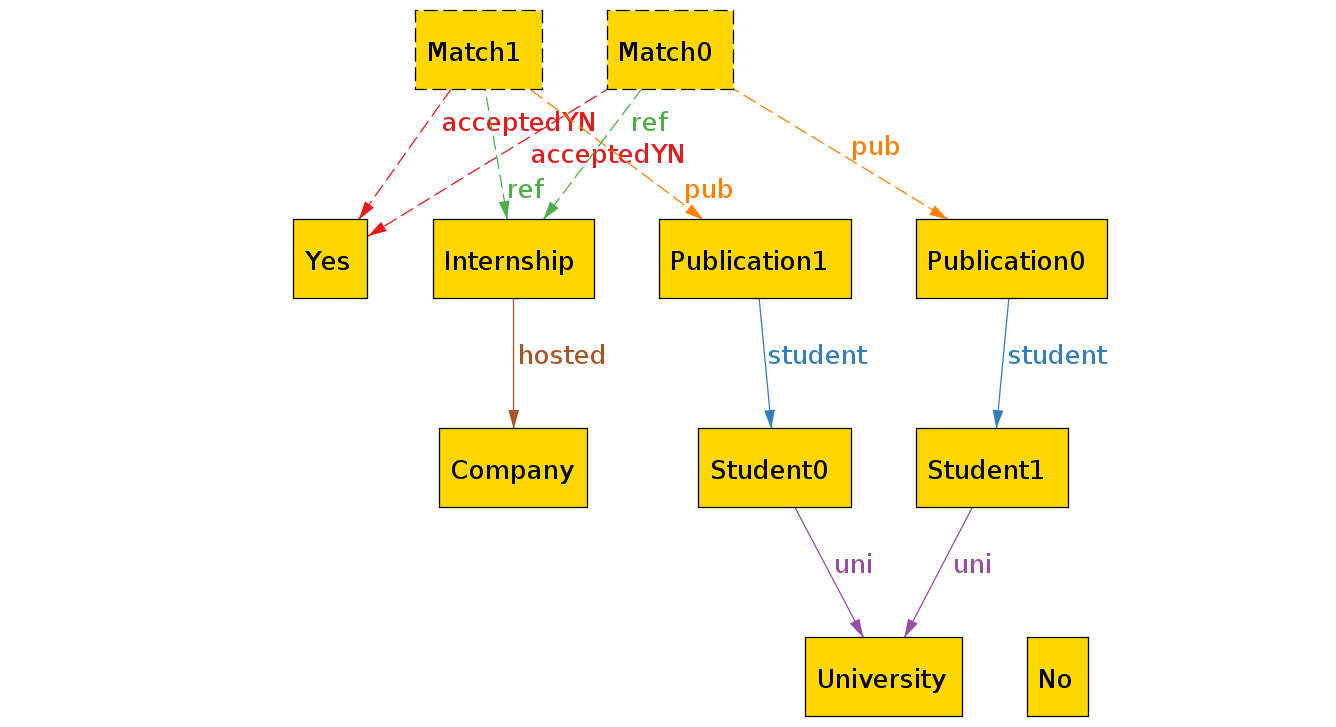
\includegraphics[width=1\linewidth]{alloy/state2.png}
    \caption{Alloy second state}
    \label{fig:state2}
\end{figure}


\begin{figure}[H]
    \centering
    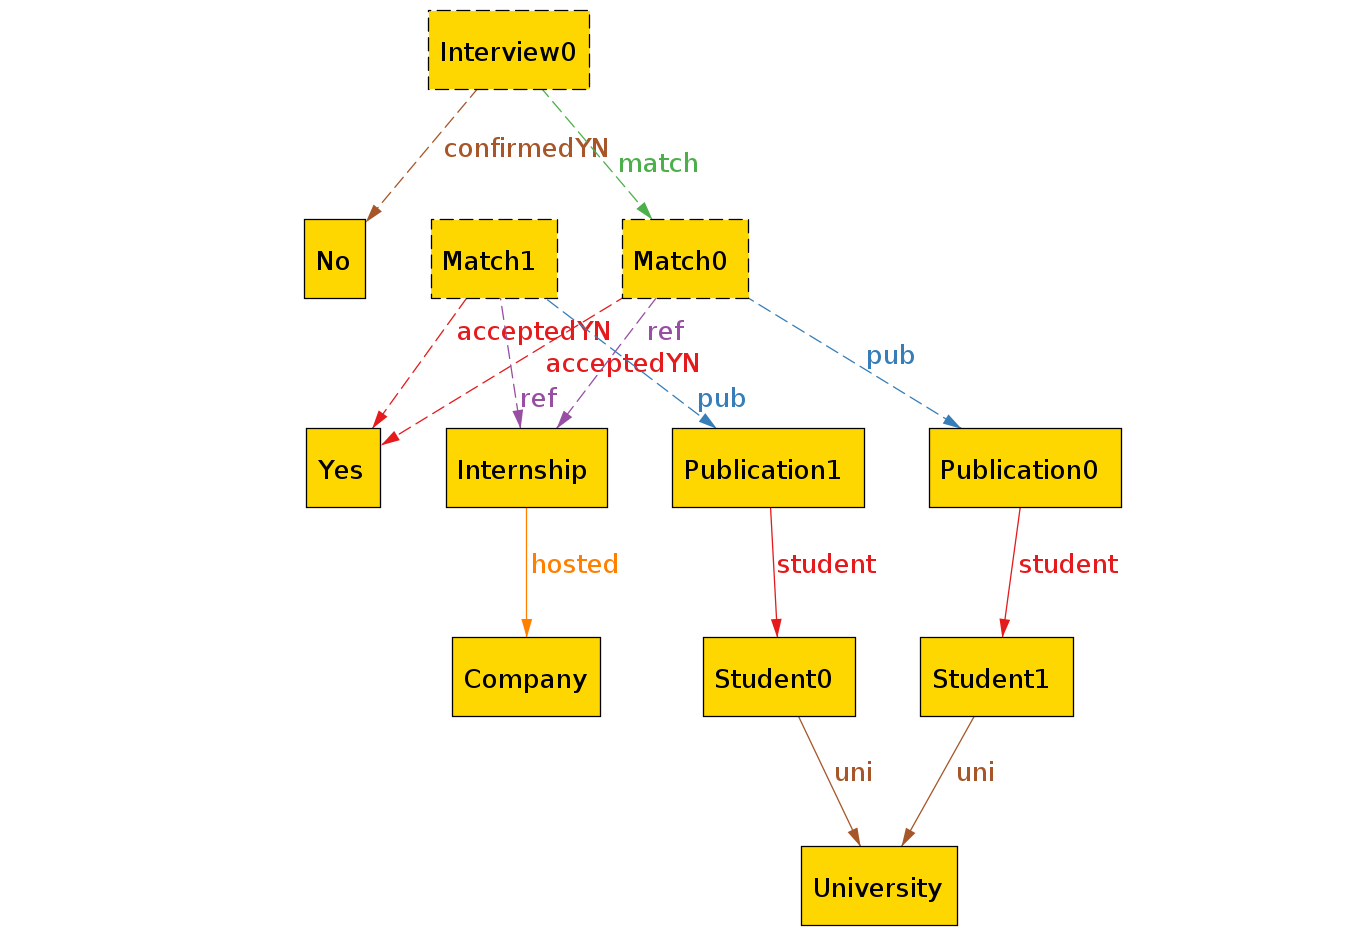
\includegraphics[width=1\linewidth]{alloy/state3.png}
    \caption{Alloy third state}
    \label{fig:state3}
\end{figure}


\begin{figure}[H]
    \centering
    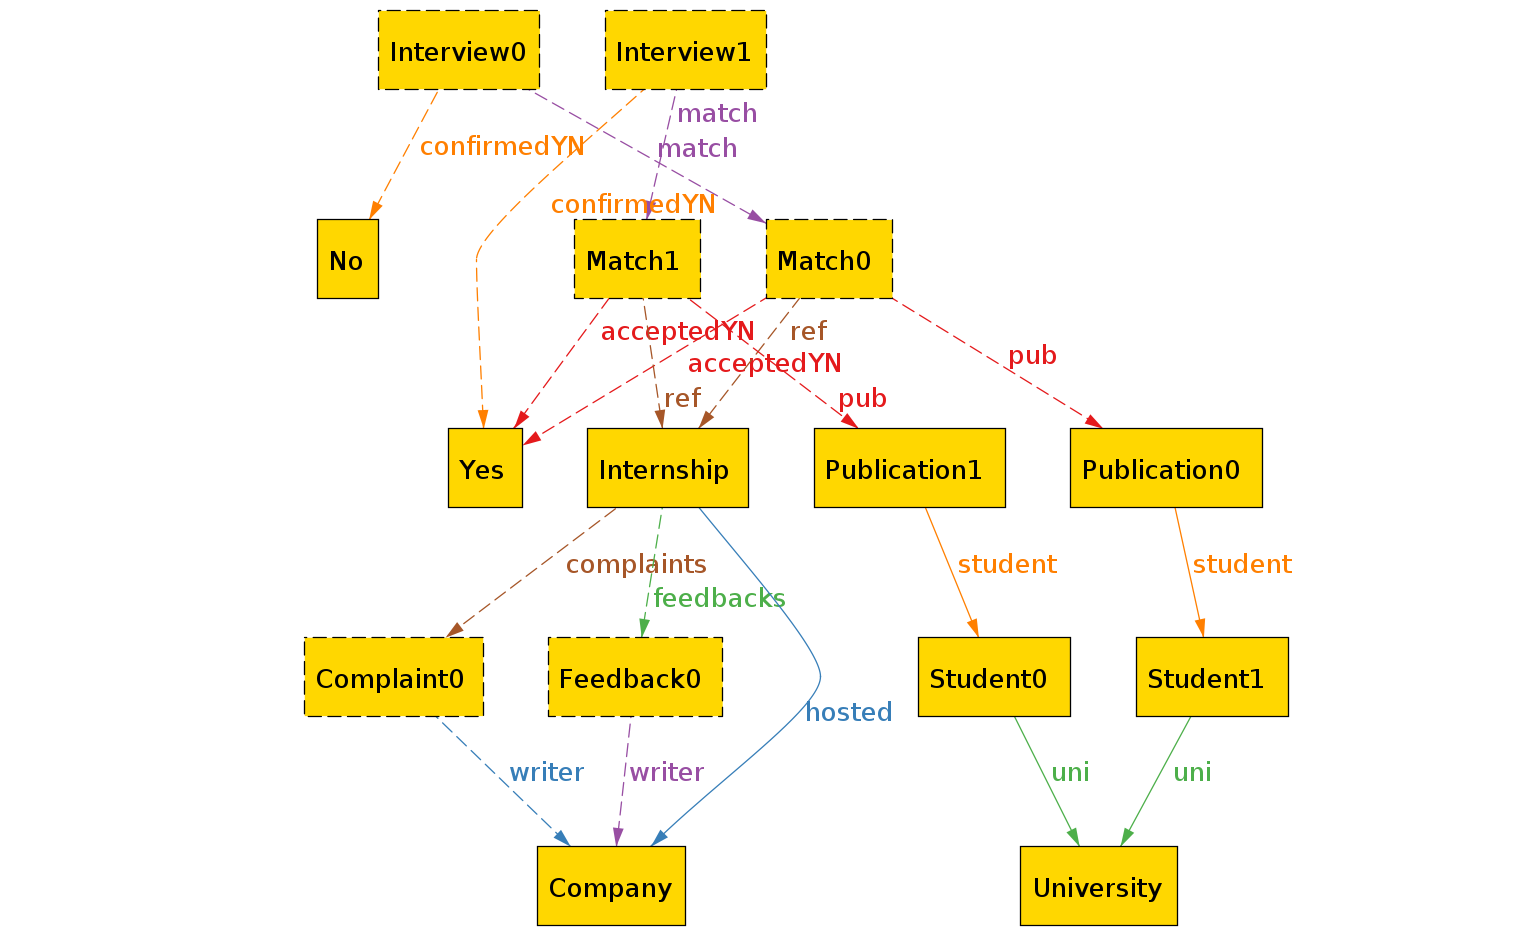
\includegraphics[width=1\linewidth]{alloy/state4.png}
    \caption{Alloy fourth state}
    \label{fig:state4}
\end{figure}

The results of the model described with alloy are showed in the images \ref{fig:state1}, \ref{fig:state2}, \ref{fig:state3} and \ref{fig:state4}; where it's possible to see the evolution of the model during the match between publications and internships, with the conducting of interviews and the creation of feedbacks and complaints.

\section{Effort Spent}
The table below show the number of hours that each member of the group worked for the RASD document.

\begin{table}[H]
    \begin{tabular}{|c|c|}
    \hline
        \textbf{Member}  & \textbf{Hours}\\ 
    \hline
        Elia Priuli &  23h\\
    \hline
        Veronica Viceconti & 24h \\
    \hline
        Marco Zuccoli & 20h \\
    \hline
    \end{tabular}
    \label{tab:my_label}
\end{table}

\section{References}

\begin{enumerate}
    \item Software Engineering II course slides
    \item Draw.io 
    \item StarUML 
    \item AlloyAnalyzer
\end{enumerate}

\end{document}